% =============================================================================
% MS MARCO Generative QA — Repository Report
% Author : GioiaZheng  <gioia.zheng.stud@gmail.com>
% Date   : 2026-07-18
% Build  : latexmk -pdf report.tex   (or:  see Makefile)
% =============================================================================

\documentclass[11pt,a4paper]{article}

% --- Encoding & language ----------------------------------------------------
\usepackage[T1]{fontenc}
\usepackage[utf8]{inputenc}
\usepackage{lmodern}
\usepackage{microtype}
% Allow line breaks inside long \texttt{} paths so the per-output
% directory names in the appendices don't push the right margin.
\usepackage{seqsplit}
\usepackage{hyphenat}
% Slightly more open vertical rhythm than article's default; paragraphs
% separated by a blank line rather than indentation (engineering-report style).
\usepackage{parskip}
\setlength{\parskip}{0.45em plus 0.15em minus 0.10em}
\renewcommand{\baselinestretch}{1.05}
% Section header polish: smaller sans-serif headings, slightly tighter
% spacing above so a section doesn't push its first paragraph too far down.
\usepackage[explicit]{titlesec}
\titleformat{\section}{\Large\bfseries}{\thesection}{0.6em}{#1}
\titleformat{\subsection}{\large\bfseries}{\thesubsection}{0.55em}{#1}
\titleformat{\subsubsection}{\normalsize\bfseries}{\thesubsubsection}{0.5em}{#1}
\titlespacing*{\section}{0pt}{1.4em plus 0.4em}{0.6em}
\titlespacing*{\subsection}{0pt}{1.0em plus 0.3em}{0.4em}
\titlespacing*{\subsubsection}{0pt}{0.8em plus 0.2em}{0.3em}
% Tighter table rule spacing.
\renewcommand{\arraystretch}{1.12}
% Global mild sloppiness: lets TeX stretch lines a little to avoid
% overfull boxes on lines with long unbreakable tokens (code paths,
% URLs, citation clusters).  Standard remedy in IEEE / ACM templates.
\setlength{\emergencystretch}{3em}

% --- Page geometry & headers ------------------------------------------------
\usepackage[a4paper,margin=2.4cm,headheight=14pt]{geometry}
\usepackage{fancyhdr}
\pagestyle{fancy}
\fancyhf{}
\fancyhead[L]{\small\nouppercase{\leftmark}}
\fancyhead[R]{\small\itshape MS~MARCO GenQA --- Repository Report}
\fancyfoot[C]{\small\thepage}
\renewcommand{\headrulewidth}{0.4pt}
\renewcommand{\footrulewidth}{0pt}
% Clean "plain" page style for the first page of each \section
% (otherwise fancyhdr puts the section header on every page including
% the title page of each chapter, which looks busy).
\fancypagestyle{plain}{%
  \fancyhf{}%
  \fancyfoot[C]{\small\thepage}%
  \renewcommand{\headrulewidth}{0pt}%
}
% Drop "Section" prefix in the running header — just the title.
\renewcommand{\sectionmark}[1]{\markboth{\thesection~~#1}{}}

% --- Math & tables ----------------------------------------------------------
\usepackage{amsmath,amssymb}
\usepackage{booktabs}
\usepackage{multirow}
\usepackage{array}
\usepackage{tabularx}
\usepackage{makecell}
\usepackage{longtable}

% --- Figures ----------------------------------------------------------------
\usepackage{graphicx}
\graphicspath{{figures/}}
\usepackage{float}
\usepackage{caption}
\captionsetup{font=small,labelfont=bf,labelsep=period}
\usepackage{subcaption}

% --- Colour (used by \todo and hyperref colorlinks) -------------------------
\usepackage{xcolor}

% --- Diagrams (pipeline schematic, forest plot) -----------------------------
\usepackage{tikz}
\usetikzlibrary{positioning,arrows.meta,shapes.geometric,fit,backgrounds}

% --- Bibliography -----------------------------------------------------------
\usepackage[backend=biber,
            style=numeric-comp,
            sorting=none,
            maxbibnames=99,
            giveninits=true,
            doi=false,isbn=false,url=false,eprint=false]{biblatex}
\addbibresource{references.bib}

% --- Hyperlinks (must be last among ref packages) ---------------------------
\usepackage[hidelinks,
            colorlinks=true,
            linkcolor=blue!55!black,
            citecolor=blue!55!black,
            urlcolor=blue!55!black,
            bookmarksnumbered=true,
            bookmarksopen=true,
            pdfpagelabels=true]{hyperref}
\usepackage[noabbrev,capitalize]{cleveref}

% --- PDF metadata -----------------------------------------------------------
\hypersetup{
  pdftitle={MS MARCO Generative QA: A Reproducible Retrieve-Rerank-Generate
            Pipeline with Grounding and Triad Audits},
  pdfauthor={GioiaZheng},
  pdfsubject={Repository report - updated 2026-08-11;
              core experiment window 2026-03-06 to 2026-05-21;
              TREC-DL external validation 2026-07-18;
              BEIR cross-domain retrieval validation 2026-07-20;
              NFCorpus and SciFact first-stage analyses;
              NFCorpus bounded query-representation
              experiment 2026-07-28},
  pdfkeywords={MS MARCO; BM25; dense retrieval; cross-encoder reranking;
               retrieval-augmented generation; BERTScore; NLI;
               RAG triad; extractive QA; paired bootstrap}
}

% --- Convenience macros -----------------------------------------------------
\newcommand{\dataset}{MS~MARCO}
\newcommand{\devsmall}{\textit{dev/small}}
\newcommand{\fdev}{6\,980}
\newcommand{\msmarco}{MS~MARCO}
\newcommand{\F}{F\textsubscript{1}}
\newcommand{\Tokenf}{Token-\F}
\newcommand{\rougel}{ROUGE-L}
\newcommand{\bertscore}{BERTScore}
\newcommand{\mrr}{MRR@10}
\newcommand{\ndcg}{nDCG@10}
\newcommand{\recallH}{Recall@100}
\newcommand{\recallK}{Recall@1000}
\newcommand{\bmtwofive}{BM25}
\newcommand{\todo}[1]{\textcolor{red}{\textbf{TODO:} #1}}
\newcommand{\delt}{$\Delta$}
\newcommand{\code}[1]{\texttt{#1}}
% Breakable arrow for prose pipelines (retrieve -> rerank -> generate).
% \to inside $...$ is a math-mode token and prevents line breaks; this
% version inserts a small skip with an explicit \allowbreak on either side.
\newcommand{\barrow}{\,\allowbreak\ensuremath{\rightarrow}\allowbreak\,}

% =============================================================================
\begin{document}

% --- Cover -------------------------------------------------------------------
\thispagestyle{empty}
\begin{titlepage}
  % Cover-local hyperref override: black, non-coloured links read as
  % typography on the cover rather than as hyperlinks.
  \hypersetup{linkcolor=black,urlcolor=black,citecolor=black,filecolor=black}
  \centering
  \vspace*{1.4cm}

  \vspace{2.6cm}

  % --- Title block ----------------------------------------------------------
  \rule{\linewidth}{1.2pt}\par
  \vspace{1.05cm}
  {\Huge\bfseries MS\,MARCO Generative QA\par}
  \vspace{0.55cm}
  {\Large\itshape A Reproducible Retrieve-Rerank-Generate Pipeline\\[0.25em]
   with Grounding and Triad Audits\par}
  \vspace{0.35cm}
   {\large Repository report - updated 2026-08-11\par}
  \vspace{1.05cm}
  \rule{\linewidth}{1.2pt}\par

  \vspace{2.8cm}

  % --- Author ---------------------------------------------------------------
  {\Large\bfseries Gioia Zheng\par}
  \vspace{0.35em}
  {\normalsize\href{mailto:gioia.zheng.stud@gmail.com}%
    {\texttt{gioia.zheng.stud@gmail.com}}\par}

  \vfill

  % --- Metadata block (framed, tighter alignment) ---------------------------
  {\renewcommand{\arraystretch}{1.30}%
   \begin{tabular}{@{}r@{\hskip 1.4em}l@{}}
     \toprule
     \textbf{Core experiment period} & 2026-03-06\,--\,2026-05-21 \quad{\small(11 milestones completed; 12-stage plan)} \\
     \textbf{External validation}     & 2026-07-18 \quad{\small(TREC-DL 2019/2020)} \\
     \textbf{Cross-domain retrieval}  & 2026-07-20 \quad{\small(BEIR NFCorpus / SciFact)} \\
     \textbf{First-stage analysis}    & 2026-07-28 \quad{\small(NFCorpus fixed-output diagnosis)} \\
     \textbf{Current update}          & 2026-07-29 \\
     \textbf{Scope}                   & Batch evaluation, CPU-only; English passage retrieval + QA \\
     \bottomrule
   \end{tabular}\par}

  \vspace{1.4cm}

  % --- Repository footer ----------------------------------------------------
  {\small\textsc{Project surfaces}\\[0.15em]
   \href{https://github.com/GioiaZheng/msmarco-genqa}%
    {\texttt{github.com/GioiaZheng/msmarco-genqa}}\\[0.12em]
   \href{https://huggingface.co/datasets/GioiaZheng/msmarco-genqa-benchmark-runs}%
    {\texttt{huggingface.co/datasets/GioiaZheng/msmarco-genqa-benchmark-runs}}\\[0.12em]
   \href{https://gioiazheng.github.io/projects/msmarco-genqa/}%
    {\texttt{gioiazheng.github.io/projects/msmarco-genqa/}}\par}

  \vspace{0.6cm}
\end{titlepage}

% --- Abstract ----------------------------------------------------------------
\newpage
\thispagestyle{empty}
\section*{Abstract}

This report documents a research-engineering project that reproduces
and analyses a complete \emph{retrieve--rerank--generate}
question-answering pipeline on the \msmarco{} Passage Ranking
benchmark~\cite{bajaj2016msmarco,nguyen2016msmarcoqa}.  Each stage is
implemented from open-source components on a single laptop, with no
GPU, no fine-tuning, and no proprietary services: \bmtwofive{}
first-stage retrieval~\cite{robertson2009bm25,lu2024bm25s} over the
8.8~million-passage corpus; a dense \texttt{Sentence-Transformers}
baseline with FAISS exact search~\cite{reimers2019sbert,johnson2019faiss}
on a qrels-anchored 50k sample; a cross-encoder
reranker~\cite{nogueira2019passage,wang2020minilm} over the top-100
candidates; and a frozen T5-small~\cite{raffel2020t5} acting as a
retrieval-augmented generator~\cite{lewis2020rag} on the top-3
retrieved passages.

The single load-bearing empirical result is a paired comparison on
all \fdev{} \devsmall{} queries: replacing \bmtwofive{} with the
cross-encoder-reranked dense top-3 as the upstream passage source ---
without touching the generator --- approximately doubles every
surface-form generation metric (\Tokenf{} $0.197 \to 0.368$, \rougel{}
$0.193 \to 0.368$), with 95\,\% paired-bootstrap
confidence intervals~\cite{koehn2004bootstrap} strictly above zero on
all four metrics.  A DistilBERT-based \bertscore{}
proxy~\cite{zhang2020bertscore,sanh2019distilbert} on a 3\,000-pair
subsample recovers the same paired $\Delta$ ($+0.173$), ruling out a
surface-form artefact.  A targeted decoding-budget sweep
($\code{max\_new\_tokens}=64\!\to\!128$) and a 40-query regression
failure taxonomy together \emph{falsify} the hypothesis that
generator truncation drives the residual regression bucket: the
generator is hitting end-of-sequence naturally on this prompt format.

A subsequent grounding audit calibrates the headline result.  Lexical
content-token grounding ($0.997$) and 3-gram grounding ($0.99$) sit
at the ceiling on both arms, showing that T5-small under the
\texttt{question: \ldots\ context: \ldots} prompt is performing
\emph{extractive} rather than truly generative QA: the rerank gain is
almost entirely downstream of retrieval.  An NLI-entailment grounding
proxy~\cite{he2023debertav3,williams2018mnli} produces the only
paired metric in the project whose sign reverses ($\Delta\!=\!-0.145$,
95\,\% CI $[-0.160,-0.130]$), most likely as an artefact of
fragmentary midword-cut outputs that defeat sentence-level NLI rather
than as a true semantic regression.

The report covers, in order: the dataset characterisation, the four
modelling stages, post-hoc evaluation layers (semantic proxy,
grounding, and the current triad diagnostic interface), an honest
comparison between the initial 12-stage
project plan and what actually shipped, and the engineering
scaffolding (reproducibility manifests, paired-bootstrap confidence
intervals, deterministic seeds) that lets every number in this
document be regenerated from one command per stage.

This 2026-07-29 update keeps the empirical claims anchored to the
original experiment outputs while bringing the repository description
up to date.  Since the experiment window closed, the project has
gained an installable CLI surface, the \texttt{rag-eval} workflow
facade, optional model-stack smoke validation, local experiment
tracking, a lightweight serving wrapper, refreshed CI, secret
scanning, a deterministic RAG triad CLI, stricter input-validation
boundaries for run files / JSONL / serving calls, and a full-corpus
TREC-DL 2019/2020 passage benchmark.  On the judged topics,
cross-encoder reranking raises MRR@10 by $+0.332$ in 2019 and
$+0.198$ in 2020 while preserving Recall@100; graded metrics agree
with an independent \texttt{ir-measures} evaluation within
$2.22\!\times\!10^{-16}$.  The same frozen reranker also improves
MRR@10 on the independent BEIR NFCorpus and SciFact collections by
$+9.18\%$ and $+3.25\%$ relative, respectively.  The unchanged
Recall@100 exposes a sharp first-stage ceiling on NFCorpus rather
than a reranker failure.

A fixed-output follow-up makes that NFCorpus ceiling more precise.
Of the 323 test queries, 72 have no judged relevant document in the
\bmtwofive{} top 100; 24 first recover a positive at ranks 101--1,000
and 48 still miss at depth 1,000.  A complete single-reviewer census
assigns 67 of the 72 failures to missing source-page context.  On the
official 102-query video subset, a predeclared comparison that changes
only the query representation raises \recallH{} from 0.2821 for the
BEIR title to 0.3700 for title plus official description
($\Delta=+0.0880$, 95\,\% paired-bootstrap CI
$[+0.0535,+0.1265]$, $p<0.0002$).  This is bounded retrieval evidence:
it neither covers the other 221 NFCorpus queries nor evaluates
generation.

\vspace{2em}
\noindent\textit{Keywords.}~~MS~MARCO; passage retrieval; \bmtwofive{};
dense retrieval; cross-encoder reranking; retrieval-augmented
generation; \bertscore{}; NLI grounding; RAG triad; paired bootstrap;
extractive QA.

\newpage
\tableofcontents
\clearpage
\listoftables
\listoffigures
\clearpage

% =============================================================================
\clearpage\section{Introduction}
\label{sec:intro}

\subsection{Background and objectives}

The project brief was to build a complete
\emph{retrieve--generate} question-answering pipeline on the
\msmarco{} corpus, exploring how each stage of the pipeline
contributes to end-to-end answer quality~\cite{bajaj2016msmarco,lewis2020rag}.
\msmarco{} is a natural target dataset for this exercise: its
queries originate from real Bing user traffic, its
relevance judgements are human-annotated, and its v2.1 Q\&A flavour
ships human-written answers that allow surface-form generation
evaluation~\cite{nguyen2016msmarcoqa}.

The brief named twelve planned milestones spanning EDA, sparse
retrieval, generation baselines, dense retrieval, reranking,
generator fine-tuning, hallucination mitigation, long-document
processing, system integration and acceleration, and a final
write-up.  In practice the project ran through eleven milestones on a
single-user, CPU-only Apple Silicon laptop, with no fine-tuning at
any stage.  \Cref{sec:plan-vs-actual} compares the plan to the actual
deliverables and explains the deviations.

\subsection{Methodological commitments}

Three principles shaped every decision the project made:

\begin{enumerate}
  \item \textbf{Honest baselines before optimisation.}  Every stage
        produces a numerically reproducible \emph{baseline} ---
        \bmtwofive{} MRR, generation \Tokenf{} on a fixed query set,
        reranking $\Delta$\mrr{} versus a precisely identified first
        stage --- before any tuning is considered.  The 200-query
        subsample baselines are clearly labelled as such; the
        load-bearing claims are restricted to the full \fdev{}
        \devsmall{} numbers.
  \item \textbf{Paired statistical tests on every comparison.}  When
        the question is ``did X help on top of Y?'' the report
        always answers it on \emph{the same query ids}, with a paired
        bootstrap~\cite{koehn2004bootstrap} reporting a 95\,\%
        confidence interval on the per-query $\Delta$, not just a
        point estimate.  When the sample is too small for that ---
        e.g.\ the 200-query smoke-test scale --- the report says so
        and labels the number as illustrative.
  \item \textbf{Calibrate metrics before celebrating them.}  Surface-
        form metrics (\rougel{}, BLEU, EM, \Tokenf{}) under-credit
        valid paraphrases~\cite{lin2004rouge,papineni2002bleu}; a
        BERTScore semantic proxy~\cite{zhang2020bertscore} and a
        grounding audit (\Cref{sec:w7}) check whether the headline
        gain is real, an artefact of overlap, or a side-effect of
        the generator's output shape.  Two of the three checks
        confirm the gain; one (the NLI proxy of \Cref{sec:w7-nli})
        flips sign, and the report devotes
        \Cref{sec:discussion-nli-flip} to that disagreement rather
        than burying it.
\end{enumerate}

\subsection{Contributions}

This report contributes the following:

\begin{itemize}
  \item A single-machine, CPU-only reproduction of the standard
        \msmarco{} Passage retrieval\barrow{}reranking\barrow{}RAG-generation
        pipeline, with the \bmtwofive{} first-stage MRR@10 within
        $\sim\!0.014$ of the published Anserini/Lucene reference
        baseline~\cite{lin2021pyserini} on the same data
        (\Cref{sec:w2}).
  \item A \emph{paired} full-dev comparison of generation quality
        under \bmtwofive{} versus cross-encoder-reranked retrieval
        (\Cref{sec:gen-x-retrieval}), with 95\,\% paired-bootstrap
        confidence intervals strictly above zero on all four
        surface-form metrics and a \bertscore{} proxy that recovers
        the same $\Delta$.
  \item A two-step \emph{falsification} of the most plausible
        explanation for the residual regression bucket
        (\Cref{sec:w6-closure}): the decoding-budget closure run and
        the grounding-ceiling reading together rule out
        \texttt{max\_new\_tokens} as the bottleneck.
  \item A grounding audit (\Cref{sec:w7}) that calibrates the rerank
        gain as a \emph{retrieval} gain almost entirely downstream of
        passage selection, and isolates a sign-reversing NLI
        anomaly (\Cref{sec:w7-nli}) most plausibly attributable to
        fragmentary outputs rather than true semantic drift.
  \item A reproducibility scaffold (per-run manifests with git
        commit, dependency hashes, command line, and per-output
        SHA-256s; deterministic seeds throughout; a single config
        file driving all four runners) sufficient to re-derive every
        number in this report from one command per stage on a
        comparable single-machine setup.
  \item A maintained repository surface around the experiments:
        installable console entry points, the \texttt{rag-eval}
        workflow facade, optional model-stack smoke validation,
        local experiment tracking with sweep-level JSON/CSV/Markdown
        summaries, rag-observatory trace/sweep exports, a lightweight
        \texttt{mgq-serve} FastAPI wrapper, CI, secret scanning, and
        separate reproducibility/security notes.
\end{itemize}

\subsection{Roadmap}

\Cref{sec:relwork} surveys the related work that anchors the design
choices.  \Cref{sec:dataset} characterises the \msmarco{} subset
actually used.  \Cref{sec:method} steps through the four modelling
stages in implementation order.  \Cref{sec:results} is the
central empirical chapter, presenting the retrieval numbers,
the load-bearing paired generation comparison, the
first-stage head-to-head, the evaluation layer, the
grounding audit, and the triad diagnostic interface.
\Cref{sec:discussion} discusses what the combination of evaluation-layer closure,
grounding, and triad diagnostics actually means about
where the gain comes from, treats the NLI sign flip on its own
terms, and compares ship versus plan.  \Cref{sec:limitations} states
the limitations.  \Cref{sec:conclusion} concludes.
The question-form breakdown is reported inline with the rest of the evaluation layer
(\Cref{tab:w6b}).  Appendices cover the configuration and
reproducibility scaffolding (\Cref{sec:reproducibility}), the full
five-way bucket counts (\Cref{sec:appendix-buckets}), and a
short glossary of cross-references (\Cref{sec:appendix-glossary}).

\subsection{Repository status as of 2026-07-29}

The project has moved from a report-centred experiment bundle to a
small research-engineering repository.  The headline metrics in this
document remain historical experiment results, but the codebase now
has a clearer operating surface:

\begin{itemize}
  \item \textbf{Workflow facade.}  \texttt{rag-eval run --config
        configs/baseline.yaml} builds or dry-runs the configured
        retrieval, reranking, generation, context-packing,
        bootstrap, grounding, and triad-evaluation workflow from one
        entry point.
  \item \textbf{Package and CLI surface.}  The project installs via
        \texttt{pip install -e .} and exposes stage-level
        \texttt{mgq-*} commands plus \texttt{mgq-serve} for local
        serving experiments.  The current evaluation surface includes
        \texttt{mgq-retrieval-report matrix} for same-qid
        \bmtwofive{} / dense / RRF / reranked comparison tables and
        \texttt{mgq-trec-eval} for an independent TREC-compatible
        metric cross-check, plus
        \texttt{mgq-context-packing-report} for packed-vs-plain
        generation prompt comparisons, plus
        \texttt{mgq-rag-triad} for context-relevance, groundedness,
        and answer-relevance diagnostics over existing generation
        outputs, plus \texttt{mgq-export-rag-observatory} and
        \texttt{mgq-export-rag-observatory-sweep} for exporting
        selected query traces and small configuration-sweep bundles to
        the observability layer.
  \item \textbf{Validation.}  Default CI runs fast pytest coverage,
        \texttt{ruff}, headline-metric metadata checks, and a
        high-confidence secret scan.  Heavy model and data checks stay
        opt-in through the model-stack smoke and slow/integration test
        markers.  A committed two-query TREC fixture validates run and
        qrels parsing, canonical export, metric scope, and agreement
        with the optional \texttt{ir-measures} backend without fetching
        the full corpus.
  \item \textbf{Reproducibility.}  The manifest contract now records
        command lines, dependency-file hashes, config hashes, git
        state, output hashes, and cache/profile metadata.  The
        documentation separates quick local checks from heavyweight
        data/model reproduction.
  \item \textbf{TREC-DL external-validity benchmark.}  The full-corpus
        \bmtwofive{} and cross-encoder runners cover all 43 judged
        topics from 2019 and all 54 from 2020, with outputs isolated
        by year.  Graded \ndcg{} and threshold-2 \mrr{} / recall
         pass independent evaluation; \Cref{sec:trec-dl-results}
         reports both tracks separately with query-level lift and
         failure analysis.
  \item \textbf{BEIR cross-domain retrieval benchmark.}  NFCorpus and
        SciFact use their own corpora and complete test qrels.  The
        unchanged top-100 cross-encoder improves \mrr{} and \ndcg{} on
        both collections; \Cref{sec:beir-results} separates that
        transfer result from the unsupported claim of full RAG
        generalization.
  \item \textbf{NFCorpus first-stage diagnosis.}  The public
        \bmtwofive{} run is now covered by a pinned data-and-metric
        contract, a complete 72-query no-hit review, and a bounded
        102-query query-representation experiment.  The result
        distinguishes omitted source context from reranker capacity
        without changing the architecture.
  \item \textbf{SciFact first-stage diagnosis.}  The matching
        fixed-output check shows a different shape: 265/300 SciFact
        queries already have a relevant top-100 candidate and 259/300
        have complete relevant-document coverage at depth 100.  This
        keeps the NFCorpus ceiling from being overgeneralised across
        all BEIR evidence.
  \item \textbf{Public evidence layer.}  Fourteen exact ranked outputs
        from TREC-DL, BEIR cross-domain, and the NFCorpus video-query
        experiment are published as checksum-verified GitHub Release
        archives and as a public Hugging Face Dataset.  The repository
        report, dataset card, and personal project page cross-link the
        same evidence boundaries.
  \item \textbf{Research backlog.}  Follow-up issues now separate
        learned sparse retrieval, stronger rerankers, chunking
        protocols, query transformation, offline/online indexing,
        citation-aware generation, and adaptive
        retrieval sufficiency checks.
\end{itemize}

% =============================================================================
\clearpage\section{Related Work}
\label{sec:relwork}

\paragraph{The \dataset{} ecosystem.}  \dataset{} is among the
largest publicly available collections of \emph{real-user} search
queries with human-judged relevance and human-written
answers~\cite{bajaj2016msmarco,nguyen2016msmarcoqa}.  Its Passage
Ranking corpus contains 8.8M passages with one or two relevance
judgements per dev query; the Q\&A v2.1 split layered on top supplies
free-form answers that make end-to-end generation tractable to
evaluate.  The benchmark has been the de-facto target for
mid-2010s-to-2020s information retrieval research; published
\bmtwofive{} baselines in the
Anserini/Lucene/Pyserini~\cite{lin2021pyserini} stack report
\mrr{}~$\approx 0.184$ on \devsmall{}.  This project's \bmtwofive{}
number (\mrr{}~$=0.170$, \Cref{sec:w2}) is within tokenizer-induced
distance of that reference.

\paragraph{Sparse retrieval.}  \bmtwofive{} remains the canonical
sparse first-stage retriever~\cite{robertson2009bm25}.  This project
uses \texttt{bm25s}~\cite{lu2024bm25s}, a pure-Python re-implementation
of the BM25 scoring formula with eager sparse scoring that achieves
Lucene-comparable throughput on commodity CPUs without requiring a
JVM; the trade-off is a different default tokenizer, which is the
main attributable source of the $\sim\!0.014$ MRR gap relative to
the Lucene-tokenizer reference baseline.

\paragraph{Dense retrieval.}  Sentence-level dense
retrievers~\cite{reimers2019sbert} encode queries and passages into a
shared embedding space.  ANCE~\cite{xiong2021ance} and subsequent
\msmarco{}-tuned encoders established that dense retrieval can
substantially outperform \bmtwofive{} on this benchmark.  This project
uses a \emph{generic} (non-domain-tuned)
\texttt{all-MiniLM-L6-v2}~\cite{wang2020minilm} encoder as the dense
baseline, deliberately leaving the \msmarco{}-tuned variant
(\texttt{msmarco-MiniLM-L6-cos-v5}) and a stronger generic encoder
(BGE small~\cite{xiao2024bge}) for the same-tier encoder comparison.  Exact
similarity search is via FAISS \texttt{IndexFlatIP}~\cite{johnson2019faiss}
on L2-normalised embeddings (cosine similarity); no approximate
nearest-neighbour index is used, since the
50k-passage sampled setting fits in memory.

\paragraph{Reranking.}  Cross-encoders applied to (query, passage)
pairs and trained on relevance labels --- the architecture introduced
by Nogueira and Cho~\cite{nogueira2019passage} --- give the highest
known single-stage reranking quality on \msmarco{}.  The reranker used
throughout this project is \texttt{cross-encoder/ms-marco-MiniLM-L-6-v2},
a small distilled cross-encoder~\cite{wang2020minilm} trained on
\msmarco{} qrels.  Reranking depth is fixed to $K\!=\!100$ throughout
the report; the K-sweep (\{50, 100, 200\}) is queued as the top-k sweep
(\Cref{sec:plan-vs-actual}).

\paragraph{Retrieval-augmented generation.}  RAG~\cite{lewis2020rag}
folds retrieved passages into the prompt of an encoder--decoder
language model.  This project's RAG generator is the smallest
T5~\cite{raffel2020t5} checkpoint (\texttt{t5-small}), used as a
frozen pretrained model with the canonical T5 extractive-QA prompt
shape (\code{question:~<q>~context:~<p1>~<p2>~<p3>}; see
\Cref{sec:w3} for the verbatim form).
The choice of T5-small is deliberate: it caps the absolute generation
quality but lets the entire pipeline run end-to-end on CPU within a
few hours per full-dev sweep, which is what makes the paired
statistical comparisons of \Cref{sec:gen-x-retrieval} possible at all.

\paragraph{Generation evaluation.}  Surface-form metrics ---
\rougel{}~\cite{lin2004rouge} and
BLEU~\cite{papineni2002bleu} --- under-credit valid paraphrases.
\bertscore{}~\cite{zhang2020bertscore} replaces n-gram overlap with
contextualised-embedding cosine similarity at the token level.  This
project uses BERTScore with a DistilBERT~\cite{sanh2019distilbert}
backbone as a \emph{semantic proxy} (deliberately not the canonical
\texttt{roberta-large} citation-grade scorer), reserving the heavier
encoder for a follow-up.  The grounding audit of \Cref{sec:w7}
borrows from the faithfulness-evaluation literature on natural
language generation~\cite{ji2023hallucination,honovich2022true},
specifically the practice of using a small NLI cross-encoder
~\cite{he2023debertav3,williams2018mnli} to score
\emph{entailment(passages $\to$ prediction)}.

\paragraph{Statistical testing.}  Every paired comparison in this
report uses Koehn's paired bootstrap~\cite{koehn2004bootstrap}
(10\,000 resamples, seed 42, percentile interval); structural
feature comparisons between regression and non-regression queries
use Mann--Whitney U with rank-biserial effect
size~\cite{mannwhitney1947}.  This is deliberate: with sample sizes
in the thousands but per-query metrics that are highly non-normal
(bimodal at 0/1 for exact-match, heavy-tailed for BLEU on short
outputs), only resampling-based intervals are credible.

% =============================================================================
\clearpage\section{Dataset and Exploratory Data Analysis}
\label{sec:dataset}

\subsection{Datasets used}

The project consumes two distinct slices of \msmarco{}:

\begin{itemize}
  \item \textbf{\msmarco{} Passage Ranking} (the retrieval corpus): 8.8M
        English passages, $\sim\!400$~bytes median length.  All
        retrieval baselines (\bmtwofive{}, dense, rerank, and
        the generator's upstream context) index this corpus.  Used
        the official \texttt{ir\_datasets}
        loader~\cite{macavaney2021irdatasets} for both the corpus and
        the \devsmall{} relevance judgements.
  \item \textbf{\msmarco{} Q\&A v2.1 validation split}: $\sim\!101$k
        queries, each with up to ten candidate passages and one or
        more human-written reference answers.  The EDA uses the
        first 5\,000 rows of this split; the generation evaluation
        uses the references attached to the \fdev{} \devsmall{}
        queries on which \bmtwofive{} and the reranker both produce a
        top-3 (\Cref{sec:gen-x-retrieval}).
\end{itemize}

\subsection{Query and passage shape}

\Cref{fig:query-length,fig:passage-length} report the empirical
length distributions on the EDA 5\,000-row validation sample.
Queries are short (median $\approx\!6$ tokens; the long tail beyond
$\sim\!15$ tokens is small), consistent with web-search behaviour;
passages are roughly $10\times$ longer (median $\approx\!50$
tokens), short enough that the generator can fit three of them
into a T5-small 512-token input window without per-passage
truncation in the common case.

\begin{figure}[H]
  \centering
  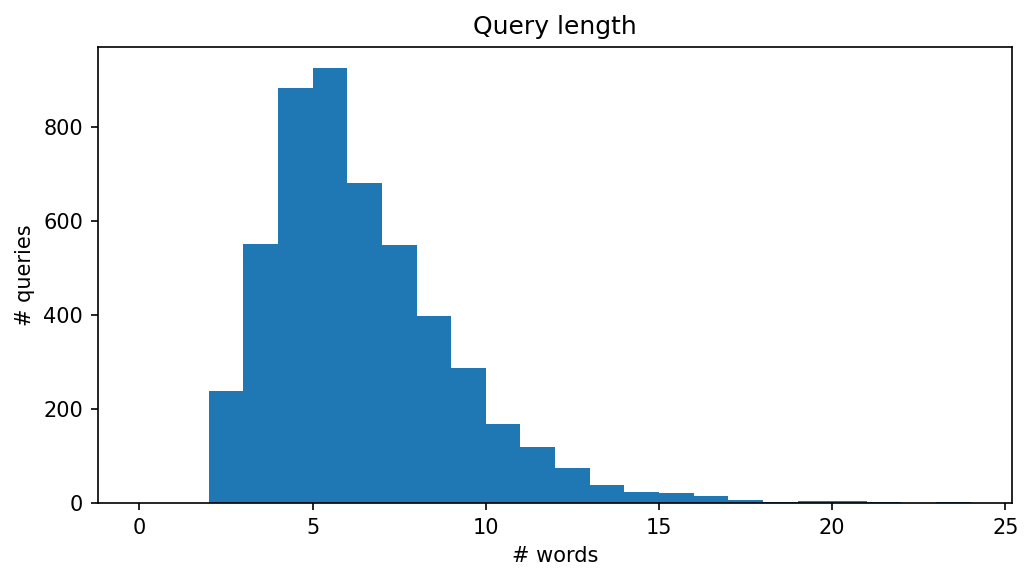
\includegraphics[width=0.78\linewidth]{figures/query_length_distribution.png}
  \caption{Query-length distribution on the EDA 5\,000-row \msmarco{}
  Q\&A v2.1 validation sample.  Median $\approx\!6$ tokens; the
  $\geq\!15$-token tail is small.  Sets the sizing target for the
  RAG prompt budget.}
  \label{fig:query-length}
\end{figure}

\begin{figure}[H]
  \centering
  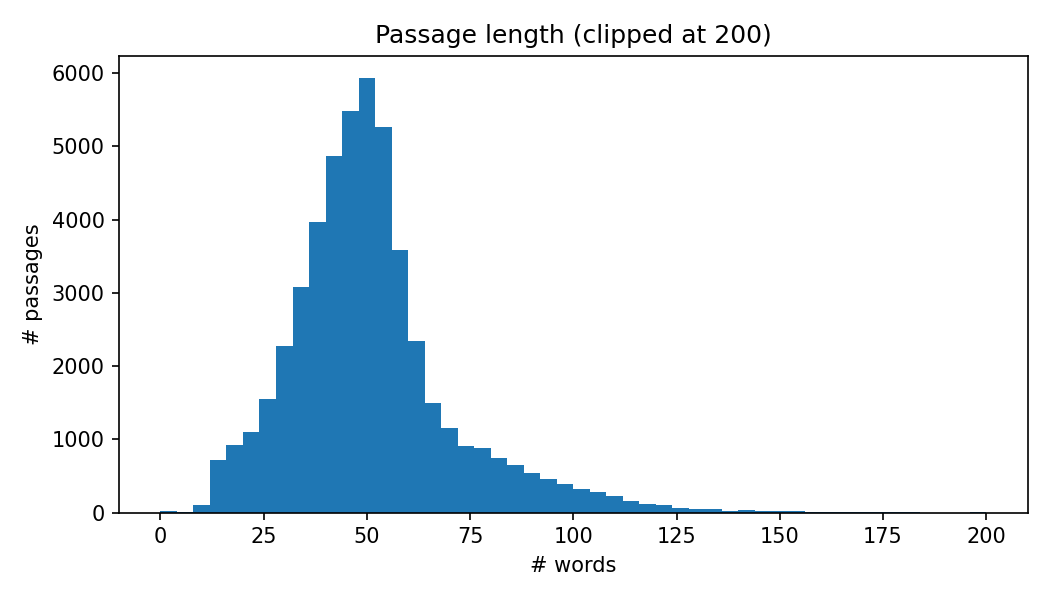
\includegraphics[width=0.78\linewidth]{figures/passage_length_distribution.png}
  \caption{Passage-length distribution on the same EDA sample,
  clipped at 200 tokens.  Median $\approx\!50$ tokens; the floor at
  one sentence is an artefact of \msmarco{}'s snippet extraction.}
  \label{fig:passage-length}
\end{figure}

\subsection{Query-type composition}

\msmarco{} ships a five-way \texttt{query\_type} label
(\texttt{DESCRIPTION}, \texttt{NUMERIC}, \texttt{ENTITY},
\texttt{LOCATION}, \texttt{PERSON}) and a separate (noisier)
free-form answer field.  On the \fdev{} \devsmall{} queries that the
load-bearing generation comparison uses, the proportions are
\texttt{DESCRIPTION}~53\,\%, \texttt{NUMERIC}~24\,\%,
\texttt{ENTITY}~9\,\%, \texttt{LOCATION}~7\,\%, \texttt{PERSON}~7\,\%
(see \Cref{tab:bucket-by-type} in \Cref{sec:gen-x-retrieval}).

\Cref{fig:query-type,fig:answer-by-type} show the EDA distributional
read on the validation sample.  Two observations end up shaping
later stages:

\begin{enumerate}
  \item \texttt{DESCRIPTION} and \texttt{NUMERIC} dominate.
        Description answers are long, free-form, and reward
        paraphrase --- which makes surface-form metrics
        (\rougel{}, BLEU, EM) systematically pessimistic on this
        class and motivates the \bertscore{} proxy
        (\Cref{sec:w6-bertscore}).  Numeric answers are short and
        rely on lexical surface match in the passage, so the
        bucket analysis of \Cref{tab:bucket-by-type} can use them
        as a sanity-check direction (numeric should gain
        \emph{less} from semantic-aware reranking than description
        does).
  \item A non-trivial fraction of queries has no answer (or an
        empty / ``no\_answer'' string).  These must be filtered for
        any supervised fine-tuning of the generator; the project
        does not run SFT, so the no-answer rows are simply scored
        through (the generator emits something, the reference is
        empty, and the metric for that row is 0).  This is honest
        but conservative.
\end{enumerate}

\begin{figure}[H]
  \centering
  
\includegraphics[width=0.78\linewidth]{figures/query_type_distribution.png}
  \caption{\msmarco{} \texttt{query\_type} label distribution on the
  EDA validation sample.  \texttt{DESCRIPTION} dominates;
  \texttt{LOCATION} and \texttt{PERSON} are smaller buckets.}
  \label{fig:query-type}
\end{figure}

\begin{figure}[H]
  \centering
  
\includegraphics[width=0.78\linewidth]{figures/answer_type_by_query_type.png}
  \caption{Answer-type composition stratified by \texttt{query\_type}.
  \texttt{DESCRIPTION} queries skew toward long free-form answers;
  \texttt{NUMERIC} queries skew toward short / single-word.}
  \label{fig:answer-by-type}
\end{figure}

\subsection{Relevance-judgement sparsity}

A subtle but consequential property of the \devsmall{} qrels:
$\geq\!95\,\%$ of dev queries have exactly one marked-relevant
passage in the 8.8M-passage corpus, and \emph{none} are negatively
labelled.  This shapes the dense-retrieval sampling design (\Cref{sec:w4}): a
uniform random 50k sample from 8.8M would leave almost no relevant
doc in the pool, so the project uses a \emph{qrels-anchored} sample
in which every dev relevant doc id is unconditionally included
alongside random distractors.  The trade-off, spelled out in
\Cref{sec:w4-sampling-caveat}, is that absolute dense/rerank metrics
on this sampled setting are upper-bounded by construction; the
\emph{within-sample} $\Delta$ between dense and \bmtwofive{} remains
the meaningful quantity.

% =============================================================================
\clearpage\section{Methodology}
\label{sec:method}

This section describes the four modelling stages (sparse retrieval,
generation, dense retrieval, and reranking) and the
post-hoc analysis layers (evaluation, grounding, triad diagnostics)
in implementation order.  All
four modelling stages ship as scripted command-line entrypoints under
\texttt{experiments/run\_*.py}, driven by a single configuration
file at \texttt{configs/baseline.yaml}; the evaluation and grounding
layers are analysis scripts
under \texttt{scripts/*.py}, the triad diagnostic is an installable
\texttt{mgq-rag-triad} diagnostic, and context packing is an installable
\texttt{mgq-context-packing-report} comparison over packed versus
plain generation predictions.  These layers write JSON / Markdown
summaries beneath the per-analysis directories under \texttt{outputs/}
(the evaluation, grounding, \texttt{rag\_triad}, and
\texttt{context\_packing} outputs).
\Cref{sec:reproducibility} documents the reproducibility scaffold.

\Cref{fig:pipeline} sketches the end-to-end flow and the place each
stage occupies in it.

\begin{figure}[H]
  \centering
  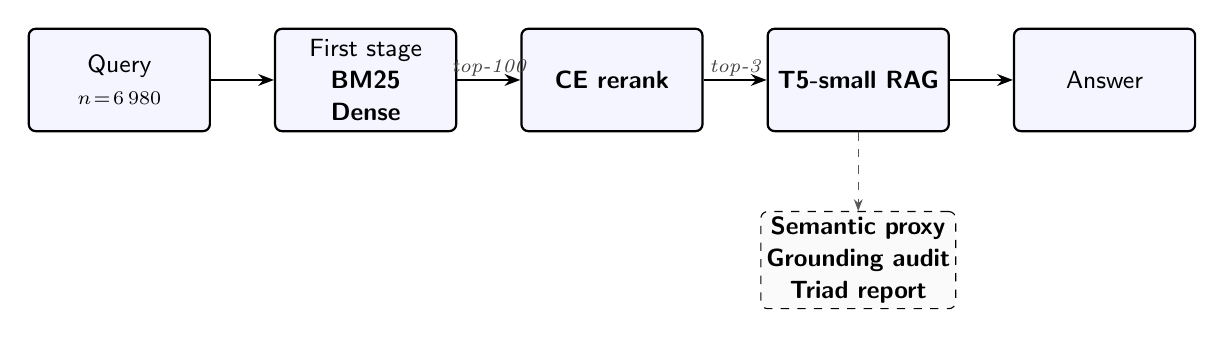
\begin{tikzpicture}[
    every node/.style={font=\small\sffamily, align=center},
    stage/.style={rectangle, draw, thick, rounded corners=2.5pt,
                  minimum width=23mm, minimum height=13mm,
                  inner sep=2pt, fill=blue!4},
    aux/.style={rectangle, draw, dashed, rounded corners=2.5pt,
                minimum width=23mm, minimum height=11mm,
                inner sep=2pt, fill=gray!4},
    flow/.style={-{Stealth[length=2mm]}, thick},
    side/.style={-{Stealth[length=1.5mm]}, dashed, gray!70!black},
    edgelbl/.style={font=\scriptsize\itshape, gray!50!black, inner sep=1pt},
  ]
    \node[stage]                              (q)   {Query\\\scriptsize $n\!=\!\fdev{}$};
    \node[stage, right=8mm of q]              (fs)  {First stage\\\textbf{BM25}\\\textbf{Dense}};
    \node[stage, right=8mm of fs]             (ce)  {\textbf{CE rerank}};
    \node[stage, right=8mm of ce]             (gen) {\textbf{T5-small RAG}};
    \node[stage, right=8mm of gen]            (ans) {Answer};

    \draw[flow] (q)   -- (fs);
    \draw[flow] (fs)  -- node[above, edgelbl] {top-100} (ce);
    \draw[flow] (ce)  -- node[above, edgelbl] {top-3}   (gen);
    \draw[flow] (gen) -- (ans);

    \node[aux, below=10mm of gen]             (eval)
      {\textbf{Semantic proxy}\\\textbf{Grounding audit}\\\textbf{Triad report}};
    \draw[side] (gen.south) -- (eval.north);
  \end{tikzpicture}
  \caption{End-to-end pipeline.  Solid boxes are the four modelling
  stages of \Cref{sec:method}; the dashed box is the post-hoc
  evaluation layer (\Cref{sec:w6,sec:w7}), plus the current triad
  diagnostic interface, which consumes the
  already-on-disk paired generation predictions and does not re-run any
  modelling stage.  BM25 and dense retrieval are interchangeable first stages
  feeding into the same downstream pipeline; the paired generation
  comparison of \Cref{sec:gen-x-retrieval} switches between them.}
  \label{fig:pipeline}
\end{figure}

\subsection{Sparse retrieval (\bmtwofive{})}
\label{sec:w2}

\paragraph{Setup.}  The first stage is \bmtwofive{} via
\texttt{bm25s}~\cite{lu2024bm25s} on the full 8.8M \msmarco{}
Passage corpus, with the canonical Robertson hyperparameters
($k_1=1.5$, $b=0.75$) and the package-default English tokenizer and
stopword list.  Index construction and query execution run
sequentially on a six-core Apple Silicon CPU; the index is persisted
to \texttt{data/processed/bm25\_index\_msmarco/} ($\approx\!2.1$~GiB)
and reused across runs.  Top-1000 candidates per query are written
to disk in TREC \texttt{run.tsv} format.

\paragraph{Retrieve pass.}  The retrieve pass over \fdev{}
\devsmall{} queries is checkpointed every 200 queries
(\texttt{retrieval.chunk\_size}) into the same \texttt{run.tsv}
target, so an interrupted run can resume at the next chunk boundary
via \texttt{--resume} without rebuilding the index or repeating
already-completed queries.  This is the only operational nicety the
project needs at retrieval scale: a single \bmtwofive{} sweep takes
$\sim\!70$~minutes on the laptop, well below the cost of the
downstream reranker, but a kill-9 mid-sweep without checkpointing
costs the full hour.

\paragraph{Evaluation.}  Retrieval metrics are computed in
\texttt{src/evaluation/retrieval.py} from the run file and the
\devsmall{} qrels.  \mrr{} follows the standard \msmarco{}
definition (reciprocal rank of the first relevant document in the
top-$10$, zero if none); \recallH{} and \recallK{} are computed at
$K\!\in\!\{100,1000\}$; \ndcg{} uses binary gain following the
standard discounted cumulative gain formulation~\cite{jarvelin2002ndcg}.

\paragraph{Independent TREC cross-check.}
The \texttt{mgq-trec-eval} boundary validates six-column run files and
binary MS MARCO qrels before exporting deterministic TREC artefacts.  It computes
\mrr{}, \ndcg{}, and \recallK{} through both the repository metric
implementation and the optional \texttt{ir-measures}
backend~\cite{macavaney2022irmeasures}.  The evaluation scope follows
TREC conventions: every query with at least one positive judgment
contributes, and a judged query absent from the run receives zero.  A
committed two-query fixture yields absolute delta 0 for all three
metrics between the two implementations.  This result validates the
adapter and metric semantics only; it does not claim that the
historical full-corpus artefacts were rerun.  Reportable \bmtwofive{},
dense, reranked, and hybrid results must each run the required external
backend against their own persisted \texttt{run.tsv}.
Graded-relevance collections are rejected rather than compared against
the repository's binary-gain \ndcg{} implementation.

\subsection{RAG generation baseline}
\label{sec:w3}

\paragraph{Generator.}  A frozen T5-small~\cite{raffel2020t5}
checkpoint, used out-of-the-box via Hugging Face
Transformers~\cite{wolf2020transformers}.  No fine-tuning at any
point.  The prompt is the canonical T5-style extractive-QA shape:
\begin{center}
  \verb|question: <q> context: <p1> <p2> <p3>|
\end{center}
where $p_1\ldots p_3$ are the top-3 passages from the upstream
retriever, ordered by descending retriever score.  Decoding uses the
T5 defaults with \texttt{max\_input\_length=512},
\texttt{max\_new\_tokens=64}; the latter is the parameter that the
evaluation-layer closure run of \Cref{sec:w6-closure} sweeps.

\paragraph{Two retrieval sources, same generator.}  The
\texttt{run\_generation\_baseline.py} runner is intentionally
\emph{retrieval-source agnostic}: it consumes any TREC-format
\texttt{run.tsv} and folds the top-$K$ passages into the prompt.
The headline generation comparison (\Cref{sec:gen-x-retrieval}) runs the
generator twice with exactly the same configuration, switching only
the upstream run between (i) the \bmtwofive{} run and (ii) the
cross-encoder-reranked dense run, and uses the runner's
\texttt{--restrict-to-run} flag to constrain both passes to the
\emph{intersection} of query ids covered by both upstream runs ---
\fdev{} queries in total, verified by query-id set-difference equal
to $\emptyset$.

\paragraph{Generation metrics.}  Four surface-form metrics: \rougel{}
via the official \texttt{rouge\_score} implementation
~\cite{lin2004rouge}, BLEU via the HF \texttt{evaluate} wrapper
around \texttt{sacrebleu}~\cite{papineni2002bleu}, exact-match, and
\Tokenf{} (lowercased, whitespace-tokenised set $F_1$).  When a
query has multiple reference answers, every metric is computed as
\emph{best-of-N over references}, which is the convention the
\msmarco{} Q\&A reference scripts use and what makes per-query
scores comparable across queries with one versus three references.

\subsection{Dense retrieval (sampled)}
\label{sec:w4}

\paragraph{Encoder \& index.}  The dense retriever uses
\texttt{\seqsplit{sentence-transformers/all-MiniLM-L6-v2}}~\cite{reimers2019sbert,wang2020minilm}
--- a generic semantic-similarity encoder, deliberately
\emph{not} \msmarco{}-tuned --- to embed both queries and passages
into a 384-dimensional space.  Embeddings are L2-normalised and
indexed with FAISS \texttt{IndexFlatIP}~\cite{johnson2019faiss}, so
inner-product search is exact cosine similarity.  No approximate
nearest-neighbour structure is used.

\paragraph{Why a sampled corpus.}
\label{sec:w4-sampling-caveat}
Encoding the full 8.8M passage corpus on a six-core CPU laptop is
prohibitive (estimated $\sim\!40$~hours at the dense encode throughput
of $16$ ms / passage).  The dense baseline therefore runs on a
\emph{50\,000-passage sample}.  A uniform random sample at this size
would put $\sim\!4\!\times\!10^{-4}\!\cdot\!8.8\textrm{M}\!\approx\!50$
relevant docs in the pool against $\sim\!17\,000$ dev relevance
judgements, so both retrievers would score near zero and the
comparison would be meaningless.  The project therefore uses a
\emph{qrels-anchored sample}: every \devsmall{} relevant doc id
(7\,437 unique docs) is included unconditionally, and the remaining
$\sim\!42\,500$ slots are filled with uniform random distractors
from the full corpus's doc\_id pool (seed 42).

\paragraph{Caveat.}  This sampling design \emph{inflates} the
absolute MRR / \ndcg{} / Recall of both retrievers, because the
relevant document is always present in the pool by construction.
The legitimate comparison is \emph{dense vs.\ \bmtwofive{} on the
same sample} (a same-pool head-to-head) --- which is exactly what
\Cref{tab:w4-results} reports.  Absolute dense numbers are \emph{not}
directly comparable to the full-corpus \bmtwofive{} number.

\paragraph{\bmtwofive{} on the same sample.}  To make the head-to-
head fair, the runner also rebuilds a \bmtwofive{} index on the same
50k-passage sample (\texttt{data/processed/bm25\_sample\_index\_50k/})
with identical hyperparameters and re-evaluates it on the same query
set.  This is the \bmtwofive{} number in \Cref{tab:w4-results}, not
the full-corpus sparse-retrieval baseline.

\subsection{Cross-encoder reranking}
\label{sec:w5}

\paragraph{Reranker.}  The reranker is
\texttt{cross-encoder/ms-marco-MiniLM-L-6-v2}~\cite{nogueira2019passage,wang2020minilm},
a small distilled \msmarco{}-trained cross-encoder.  It scores
$(\text{query}, \text{passage})$ pairs jointly --- as opposed to the
dense bi-encoder which encodes them independently --- producing a
relevance score for each of the top-$K$ candidates from the first
stage.

\paragraph{Depth.}  Throughout the report, $K\!=\!100$
(\texttt{reranker.rerank\_top\_k}).  The choice is empirically
motivated and operationally pragmatic: $K\!=\!100$ is the standard
\msmarco{} reranking depth in the literature and balances rerank
quality against wall-clock cost, which is linear in $K$.  The
K-sweep ($\{50, 100, 200\}$) is queued as the top-k sweep and explicitly
de-scoped per the project's reduced-scope deadline
(\Cref{sec:plan-vs-actual}).

\paragraph{Two arms.}  Two rerank runs are reported: one over the
dense top-100 (\Cref{sec:w5-dense-rerank}, the canonical setup) and
one over the \bmtwofive{} top-100 (\Cref{sec:w5a}, the first-stage
head-to-head against the dense arm).  Both use the same reranker
checkpoint, the same depth, and the same evaluation pass.

\paragraph{Cost.}  The dense+rerank full-dev run takes
$\approx\!4$~h~$37$~min on a 6-core MacBook CPU
(538\,000 (query, passage) pairs at $\sim\!32$~pairs/s, peak RSS
$\sim\!3.3$~GiB); the \bmtwofive{}+rerank arm takes
$\approx\!3$~h~$43$~min.  The cross-encoder is by far the slowest
stage in the pipeline.

\subsection{Evaluation layer}
\label{sec:w6-method}

The evaluation layer adds two post-hoc analyses on the already-on-disk paired
generation predictions, neither of which requires re-running the generator or reranker:

\paragraph{Semantic-proxy \bertscore{}.}  A DistilBERT-based
\bertscore{}~\cite{zhang2020bertscore,sanh2019distilbert} is
computed on a 3\,000-pair subsample of the shared qid set
(seed 42 deterministic), with
\texttt{rescale\_with\_baseline=True} and multi-reference max-$F_1$
per query.  This is a deliberate \emph{proxy}: the canonical
\texttt{roberta-large} \bertscore{} is reserved for a follow-up
(citation-grade, $\sim\!$hours of CPU on full dev).  The proxy's
sole purpose is to answer ``does the rerank $\Delta$ also show up in
a semantic-similarity scorer?''

\paragraph{Regression failure taxonomy.}  A 40-query seeded triage
(seed 42) over the \emph{regression bucket} of \Cref{sec:gen-x-retrieval}
--- 233 queries on which the reranker brought the relevant passage
into the generator's top-3 \emph{yet} \Tokenf{} dropped versus
\bmtwofive{}.  Labels are produced by a deterministic five-way rule
cascade (\texttt{scripts/regression\_failure\_taxonomy.py}); first
match wins.  Categories: \texttt{truncation\_short},
\texttt{truncation\_midword}, \texttt{topic\_drift},
\texttt{extractive\_passage\_bias}, \texttt{semantic\_mismatch} ---
the last is the residual catch-all.

\paragraph{Decoding-budget closure.}  A targeted full-dev sweep at
\texttt{max\_new\_tokens=128} (vs.\ the canonical 64), holding the
generator, prompts, retrieval inputs, and seed fixed.  Outputs are
written to fresh \texttt{\_mnt128} directories; the canonical
\texttt{\_full} predictions are untouched.  Same paired-bootstrap CI
machinery is then applied to the new predictions.

\paragraph{Question-form breakdowns.}  Three offline analyses on the
per-query metric tables: (A) a syntactic question-form tagger over
all \fdev{} queries (who / what / when / where / why / how / which
/ yes\_no / other), (B) per-form \Tokenf{} / \rougel{} / EM /
\mrr{} / \ndcg{} $\Delta$ with paired-bootstrap CIs, and (C) a
Mann--Whitney U comparison~\cite{mannwhitney1947} of five structural
features between regression and non-regression queries.

\subsection{Grounding audit}
\label{sec:w7-method}

The grounding audit is the project's faithfulness layer.  The leading question is:
\emph{is T5-small extracting content from the retrieved passages, or
generating from its parametric memory and happening to overlap?}

\paragraph{Lexical content-token grounding.}  For each prediction,
compute the fraction of unique non-stopword tokens in the prediction
(lowercased) that appear anywhere in the union of the prompt's
top-3 passages.  A local 85-word stopword list keeps the metric
self-contained.  A score of $1.0$ means every distinct content word
the model emitted is present in one of the passages it was
conditioned on; the metric is bag-of-content-tokens.

\paragraph{3-gram grounding.}  Tighter than the lexical metric:
fraction of the prediction's contiguous 3-grams (case-folded,
stopwords retained --- order is the signal) that appear as a
contiguous span in at least one passage.  Catches ``the model strung
together the right words in the wrong order'' cases the bag-of-
content-tokens score misses.

\paragraph{NLI-entailment grounding.}  An NLI cross-encoder
(\texttt{\seqsplit{cross-encoder/nli-deberta-v3-small}}~\cite{he2023debertav3,williams2018mnli})
scores \emph{entailment}$(\text{passages} \to \text{prediction})$ on
the same 3\,000-paired-qid subsample used by the \bertscore{}
proxy.  Same paired-bootstrap-CI machinery.  This is the semantic-
faithfulness companion to the two lexical grounding metrics.

\paragraph{Edge cases.}  Predictions with no content tokens score
lexical $1.0$ vacuously; predictions shorter than $n\!=\!3$ tokens
score 3-gram $1.0$ vacuously.  Both counts are reported per arm so
the convention cannot silently inflate the headline number; in
practice the vacuous shape is identical on both arms, so the paired
$\Delta$ is unaffected.

% =============================================================================
\clearpage\section{Results}
\label{sec:results}

This section reports results in the order in which they were
produced: the per-stage retrieval baselines (sparse, dense, rerank,
\Cref{sec:w2-results,sec:w4-results,sec:w5-dense-rerank}), the
paired generation comparison that constitutes the principal
empirical finding (\Cref{sec:gen-x-retrieval}), the first-stage
$\times$ reranker head-to-head (\Cref{sec:w5a}), and the
two post-hoc calibration layers --- semantic-proxy evaluation
(\Cref{sec:w6}) and grounding audit (\Cref{sec:w7}).
\Cref{sec:discussion} integrates the findings.

\subsection{\bmtwofive{} baseline (full corpus)}
\label{sec:w2-results}

\Cref{tab:w2-results} reports the \bmtwofive{} numbers on the full
8.8M-passage corpus and \fdev{} \devsmall{} queries, against the
published Anserini/Lucene reference.

\begin{table}[H]
  \centering
  \caption{\bmtwofive{} on the full \msmarco{} Passage corpus,
  \fdev{} \devsmall{} queries.  Reference: published Anserini/Lucene
  \mrr{}~$\approx 0.184$~\cite{lin2021pyserini}.  The $\sim\!0.014$
  gap is attributable to tokenizer differences between Lucene's
  \texttt{EnglishAnalyzer} and the \texttt{bm25s} package
  default.}
  \label{tab:w2-results}
  \begin{tabular}{lr}
    \toprule
    Metric        & Value \\
    \midrule
    \mrr{}        & 0.1703 \\
    \ndcg{}       & 0.2138 \\
    \recallH{}    & 0.6212 \\
    \recallK{}    & 0.8154 \\
    \bottomrule
  \end{tabular}
\end{table}

The \recallH{}~$=0.621$ number deserves attention because it caps
what any reranker on top of \bmtwofive{} can achieve in \mrr{} /
\ndcg{}: on $\sim\!38\,\%$ of \devsmall{} queries, the relevant
passage is not in the \bmtwofive{} top-100 \emph{at all}.  This
recall ceiling is what makes the constrained-recovery comparison in
\Cref{sec:w5a} non-trivial.

\subsection{Dense vs.\ \bmtwofive{} on the same sample}
\label{sec:w4-results}

\Cref{tab:w4-results} reports the dense baseline against
\bmtwofive{} rebuilt on the \emph{same} qrels-anchored 50k sample.
Both columns evaluate on the same \fdev{} queries.

\begin{table}[H]
  \centering
  \caption{Dense vs.\ \bmtwofive{} on the same
  qrels-anchored 50k passage sample, \fdev{} \devsmall{} queries.
  Encoder: \texttt{sentence-transformers/all-MiniLM-L6-v2} (generic,
  not \msmarco{}-tuned).  Index: FAISS \texttt{IndexFlatIP} over
  L2-normalised embeddings.  Absolute numbers are upper-bounded by
  the qrels-anchored sampling design (\Cref{sec:w4-sampling-caveat});
  the meaningful comparison is the same-sample $\Delta$.}
  \label{tab:w4-results}
  % Refresh with: python scripts/export_report_tables.py
\begin{tabular}{lrrr}
    \toprule
    Metric & \bmtwofive{} (sample) & Dense (sample) & $\Delta$ (dense $-$ \bmtwofive{}) \\
    \midrule
    \mrr{} & 0.6948 & 0.8830 & $+0.1882$ \\
    \ndcg{} & 0.7270 & 0.9041 & $+0.1771$ \\
    \recallH{} & 0.9338 & 0.9946 & $+0.0608$ \\
    \recallK{} & 0.9686 & 0.9991 & $+0.0305$ \\
    \bottomrule
\end{tabular}

\end{table}

Two observations:

\begin{enumerate}
  \item Dense wins on every metric on the same pool.  The
        \mrr{}~$\Delta\!=\!+0.19$ is the largest single-step gain in
        the pipeline; consistent with the literature that generic
        dense encoders close most of the semantic-matching gap that
        \bmtwofive{} leaves open, even without
        \msmarco{}-specific tuning.
  \item Dense \recallH{}~$=0.9946$ is effectively at the ceiling on
        this sampled setting.  From reranking onward, recall is no longer
        the bottleneck; the reranker's job is to tighten
        \emph{local ordering} (rank-1 vs.\ rank-3 vs.\ rank-10) given
        that the relevant passage is already in the top-100.
\end{enumerate}

\subsection{Encoder horizontal on the dense sample}
\label{sec:w4b}

\Cref{tab:w4b-encoders} compares three same-tier general-purpose
encoders on the identical dense 50k qrels-anchored sample.  All three
runs share the same sample selection, same BM25-on-sample baseline,
and the same evaluation pool, so the comparison is apples-to-apples.

\begin{table}[H]
  \centering
  \caption{Same-tier dense encoders on the dense 50k
  qrels-anchored sample.  Encoding throughput (ms/passage) measured
  on a single CPU process. Best per column in \textbf{bold}.}
  \label{tab:w4b-encoders}
  \resizebox{\linewidth}{!}{%
  \begin{tabular}{lrrrrr}
    \toprule
    Encoder & \mrr{} & \ndcg{} & \recallH{} & \recallK{} & ms/passage \\
    \midrule
    \texttt{all-MiniLM-L6-v2} (dense baseline) & 0.8830 & 0.9041 & 0.9946 & 0.9991 & \textbf{16.2} \\
    \texttt{all-MiniLM-L12-v2}              & 0.8933 & 0.9131 & 0.9955 & \textbf{0.9996} & 31.3 \\
    \texttt{BAAI/bge-small-en-v1.5}         & \textbf{0.9021} & \textbf{0.9196} & \textbf{0.9967} & 0.9994 & 34.4 \\
    \bottomrule
  \end{tabular}%
  }
\end{table}

\paragraph{Read.}  bge-small-en-v1.5 lifts \mrr{} by $+0.019$ over
the dense baseline at $\sim\!2\!\times$ encoding cost (CPU,
ms/passage).  MiniLM-L12 sits in the middle on both axes
($+0.010$ \mrr{} for the same $\sim\!2\!\times$ cost as bge-small).
The throughput / quality trade is close to linear in this tier;
none of the three encoders dominates strictly.  The density-sensitivity
sweep (\Cref{sec:w4a}) uses bge-small as the encoder.

\subsection{Density sensitivity of the dense vs.\ \bmtwofive{} gap}
\label{sec:w4a}

The dense 50k baseline is one point on a wider trade-off:
\emph{how does the dense-vs-\bmtwofive{} gap shift as the sample
dilutes?}  \Cref{tab:w4a-density} sweeps three sample sizes (15k,
30k, 50k) with bge-small (the encoder-comparison winner) and the same BM25-on-sample
baseline at each size.

\begin{table}[H]
  \centering
  \caption{Density sensitivity of the same-sample
  BM25-vs-dense gap. Encoder: \texttt{BAAI/bge-small-en-v1.5}
  (encoder-comparison winner). Density is the share of the sample that is
  relevant to $\geq\!1$ \devsmall{} query --- qrels-anchored
  sampling unconditionally includes every dev relevant doc, then
  fills with distractors, so density falls monotonically as the
  sample grows.}
  \label{tab:w4a-density}
  \resizebox{\linewidth}{!}{%
  \begin{tabular}{lrrrrr}
    \toprule
    Sample & Density & \bmtwofive{} \mrr{} & Dense \mrr{} & $\Delta$ (dense $-$ \bmtwofive{}) & Dense \recallH{} \\
    \midrule
    15k & 49.6\,\% & 0.7806 & 0.9470 & $+0.1664$ & 0.998 \\
    30k & 24.8\,\% & 0.7349 & 0.9232 & $+0.1883$ & 0.998 \\
    50k & 14.9\,\% & 0.6948 & 0.9021 & $\mathbf{+0.2074}$ & 0.997 \\
    \bottomrule
  \end{tabular}%
  }
\end{table}

\begin{figure}[H]
  \centering
  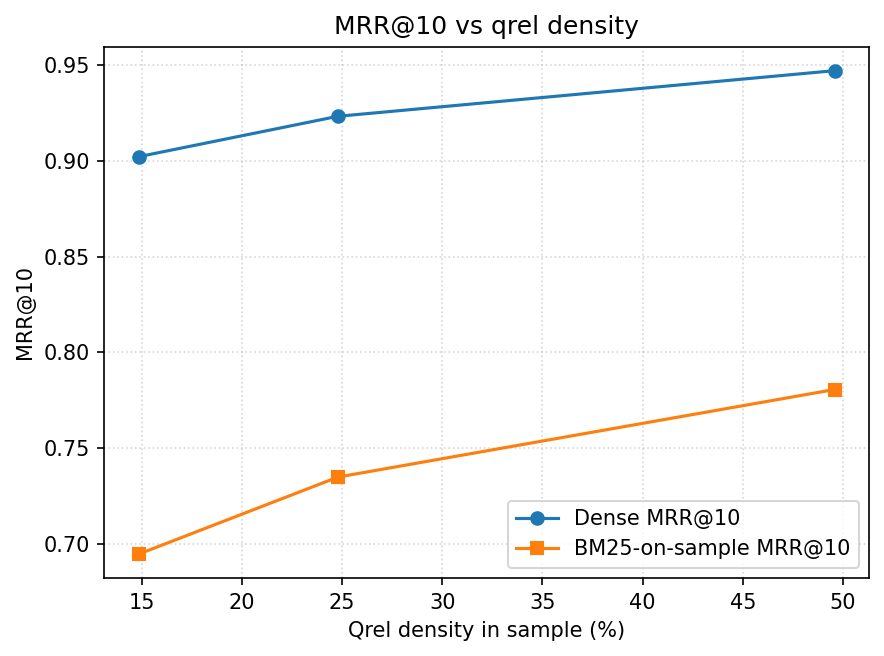
\includegraphics[width=0.78\linewidth]{figures/dense_vs_bm25_density_curve.png}
  \caption{\mrr{} vs.\ qrel-density on the same three
  qrels-anchored samples as \Cref{tab:w4a-density}.  Encoder:
  \texttt{BAAI/bge-small-en-v1.5}.  Density decreases left-to-right
  (50k sample on the left at $\sim\!15\,\%$, 15k sample on the
  right at $\sim\!50\,\%$).  The dense-vs-\bmtwofive{} gap widens
  monotonically as density drops --- which is the load-bearing
  read; absolute \mrr{} levels are inflated by the qrels-anchored
  sampling design (\Cref{sec:w4-sampling-caveat}) on every row.}
  \label{fig:w4a-density-curve}
\end{figure}

\paragraph{Read.}  As the sample grows (density drops), dense's
advantage over \bmtwofive{} grows monotonically: $+0.166 \to +0.188
\to +0.207$ (\Cref{fig:w4a-density-curve} shows the two arms
diverging visibly).  This is consistent with the literature claim
that \bmtwofive{} is competitive at high relevant-density and loses
headroom to a generic dense encoder as the distractor mass dilutes
the pool.  The trend is informative even though the absolute
density range (15\,\%--50\,\%) is much higher than the 1/5/10\,\%
the project plan originally targeted --- those cells need 70k--700k
samples to reach (dev/small has $\sim\!7{,}437$ unique relevant
doc ids, so a true 1\,\% density needs a $\sim\!700{,}000$-passage
sample) and are deferred.

\subsection{Cross-encoder reranking on the dense top-100}
\label{sec:w5-dense-rerank}

\Cref{tab:w5-results} reports the cross-encoder reranking of the
dense top-100, on the full \fdev{} \devsmall{} queries.

\begin{table}[H]
  \centering
  \caption{Cross-encoder reranking of the dense top-100,
  \fdev{} \devsmall{} queries.  Reranker: \texttt{cross-encoder/
  ms-marco-MiniLM-L-6-v2} at depth $K\!=\!100$.  Recall@100 is
  unchanged by construction (the reranker is order-only).  The
  earlier 1\,000-query subsample produced consistent deltas
  (MRR $\Delta\!=\!+0.0435$, nDCG $\Delta\!=\!+0.0398$), so the
  full-dev gain is not a subsample artefact.}
  \label{tab:w5-results}
  % Refresh with: python scripts/export_report_tables.py
\begin{tabular}{lrrr}
    \toprule
    Metric & Dense & Dense $+$ CE rerank & $\Delta$ \\
    \midrule
    \mrr{} & 0.8830 & 0.9304 & $\mathbf{+0.0474}$ \\
    \ndcg{} & 0.9041 & 0.9434 & $+0.0393$ \\
    \recallH{} & 0.9946 & 0.9946 & $\phantom{+}0.0000$ \\
    \bottomrule
\end{tabular}

\end{table}

The reranker buys $\sim\!+0.05$ MRR even with recall saturated: it
is doing exactly what \Cref{sec:w4-results} predicted it should ---
moving the relevant passage from rank 2--3 to rank 1.  Wall-clock
cost: $\approx 4$~h~$37$~min on the laptop;
peak RSS $\approx 3.3$~GiB.  The cross-encoder is the slowest stage
in the pipeline by approximately two orders of magnitude.

\subsection{TREC-DL full-corpus external-validity benchmark}
\label{sec:trec-dl-results}

The sampled dense results above cannot establish full-corpus external
validity.  The TREC-DL experiment therefore holds the architecture
fixed and changes only the independently judged topic set: the same
8,841,823-passage \bmtwofive{} index retrieves top-1,000 candidates,
and the same \texttt{cross-encoder/ms-marco-MiniLM-L-6-v2} revision
reranks the top-100.  \ndcg{} keeps the original 0--3 labels; \mrr{}
and recall treat labels 2--3 as relevant.

\begin{table}[H]
  \centering
  \caption{Full-corpus \bmtwofive{} versus \bmtwofive{} plus
  cross-encoder reranking on all 43 judged TREC-DL 2019 passage
  topics.  The reranked run contains top-100 only, so its
  \recallK{} is not reported.}
  \label{tab:trec-dl-2019}
  % Refresh with: python scripts/export_report_tables.py
\begin{tabular}{lrrr}
    \toprule
    Metric & \bmtwofive{} & \bmtwofive{} $+$ CE & $\Delta$ \\
    \midrule
    \mrr{} & 0.5471 & 0.8787 & $\mathbf{+0.3315}$ \\
    \ndcg{} & 0.4239 & 0.7210 & $\mathbf{+0.2971}$ \\
    \recallH{} & 0.4469 & 0.4469 & $\phantom{+}0.0000$ \\
    \recallK{} & 0.6983 & n/a (top-100) & n/a \\
    \bottomrule
\end{tabular}

\end{table}

\begin{table}[H]
  \centering
  \caption{The same frozen full-corpus protocol on all 54 judged
  TREC-DL 2020 passage topics.}
  \label{tab:trec-dl-2020}
  % Refresh with: python scripts/export_report_tables.py
\begin{tabular}{lrrr}
    \toprule
    Metric & \bmtwofive{} & \bmtwofive{} $+$ CE & $\Delta$ \\
    \midrule
    \mrr{} & 0.6280 & 0.8256 & $\mathbf{+0.1976}$ \\
    \ndcg{} & 0.4773 & 0.6801 & $\mathbf{+0.2027}$ \\
    \recallH{} & 0.5105 & 0.5105 & $\phantom{+}0.0000$ \\
    \recallK{} & 0.7521 & n/a (top-100) & n/a \\
    \bottomrule
\end{tabular}

\end{table}

The ordering gain repeats across both tracks: \mrr{} increases by
$+0.3315$ in 2019 and $+0.1976$ in 2020; graded \ndcg{} increases by
$+0.2971$ and $+0.2027$, respectively.  Recall@100 is unchanged by
construction because the reranker does not introduce documents.
Every run covers its complete judged-topic set.  Independent
\texttt{ir-measures}~0.4.3 evaluations agree with the internal
metrics to at most $2.22\!\times\!10^{-16}$, well inside the
$10^{-12}$ tolerance.

The query-level read is consistent with an order-only mechanism.
In 2019, 21 topics are promoted, two become new top-10 hits, one is
demoted, and none loses a top-10 hit; the 2020 counts are 18, three,
three, and zero.  The unchanged misses (one in 2019, four in 2020)
remain first-stage failures that reranking cannot repair.  Several
demotions expose judgment granularity rather than an unambiguous
semantic error: for the 2020 query ``is caffeine a narcotic'', CE
ranks an explicit negative answer first, but that passage is labelled
0 while a passage about a caffeine/codeine combination drug is
labelled 3.  This is why the report retains both graded metrics and
thresholded case review.

The cold full-index run took 602.3~s; cached-index search took 18.5~s
for 2019 and 20.9~s for 2020.  CPU reranking took 98.9~s for 4,300
pairs (43 pairs/s) and 91.8~s for 5,400 pairs (59 pairs/s).  Exact
metrics, configuration, artifact hashes, and table provenance are
recorded in \texttt{reports/generated/artifacts/
trec\_dl\_bm25\_ce.json}.

\subsection{BEIR cross-domain retrieval benchmark}
\label{sec:beir-results}

TREC-DL changes the judged queries but retains the MS~MARCO passage
collection.  To test transfer beyond that corpus without changing the
architecture, the same \bmtwofive{} configuration and frozen MiniLM
cross-encoder were run on the BEIR NFCorpus medical test collection
and the SciFact scientific-claim test collection
~\cite{thakur2021beir,boteva2016nfcorpus,wadden2020scifact}.  Each run uses its
dataset's own full corpus and graded qrels; binary MRR and recall count
labels $\geq 1$ as relevant, while \ndcg{} retains the graded labels.

\begin{table}[H]
  \centering\small
  \caption{Full-corpus \bmtwofive{} and fixed top-100 cross-encoder
  reranking on all 323 NFCorpus and 300 SciFact test queries.  The
  reranked files have depth 100, so \recallK{} is not applicable.}
  \label{tab:beir-cross-domain}
  % Refresh with: python scripts/export_report_tables.py
\begin{tabular}{llrrrr}
    \toprule
    Dataset & System & \mrr{} & \ndcg{} & \recallH{} & \recallK{} \\
    \midrule
    NFCorpus & \bmtwofive{} & 0.5186 & 0.3064 & 0.2378 & 0.4572 \\
    NFCorpus & \bmtwofive{} $+$ CE & 0.5662 & 0.3411 & 0.2378 & n/a \\
    SciFact & \bmtwofive{} & 0.6312 & 0.6617 & 0.8759 & 0.9606 \\
    SciFact & \bmtwofive{} $+$ CE & 0.6517 & 0.6787 & 0.8759 & n/a \\
    \bottomrule
\end{tabular}

\end{table}

The direction of the ranking effect transfers to both collections.
On NFCorpus, \mrr{} rises from 0.5186 to 0.5662 ($+9.18\%$ relative)
and \ndcg{} from 0.3064 to 0.3411 ($+11.33\%$).  On SciFact, the
corresponding changes are 0.6312 to 0.6517 ($+3.25\%$) and 0.6617 to
0.6787 ($+2.56\%$).  Recall@100 remains exactly unchanged because CE
only reorders the candidate set.

The more important diagnostic is first-stage coverage.  NFCorpus
\recallH{} is only 0.2378, versus 0.8759 on SciFact; therefore most
NFCorpus relevant documents never reach the reranker.  Improving the
first-stage retriever is the evidence-led next experiment for that
collection.  This is a two-dataset retrieval-transfer result, not a
claim that the complete RAG pipeline or its generator generalizes
across domains.

All 623 judged queries are present.  Structural checks found no
malformed rows, duplicate documents, rank gaps, non-finite scores, or
candidate-set changes.  Independent \texttt{ir-measures} evaluation
agrees within $4.45\!\times\!10^{-16}$.  CPU reranking took 3,110.1~s
for 32,300 NFCorpus pairs and 2,393.6~s for 30,000 SciFact pairs.  The
machine contained an NVIDIA GPU, but both recorded Python environments
used CPU-only PyTorch; these are therefore CPU timings.  Exact metrics,
commits, model revision, runtimes, and artifact hashes are recorded in
\texttt{reports/generated/artifacts/
beir\_cross\_domain\_bm25\_ce.json}.

The exact four ranked outputs are also pinned by
\texttt{artifacts/beir\_cross\_domain\_v1.json} and published as a
checksummed, text-only GitHub Release bundle.  Running
\texttt{make reproduce-beir-eval} verifies the archive and every member,
recovers the public test qrels through \texttt{ir\_datasets}, and recomputes
all four rows without rebuilding either corpus index or rerunning the
cross-encoder.  The bundle excludes document and query text, qrels mirrors,
model weights, caches, and machine-local manifests.

\subsection{SciFact first-stage diagnosis}
\label{sec:scifact-first-stage}

The SciFact aggregate result above is not just a smaller reranking
gain; it reflects a different first-stage coverage shape.  A
fixed-output diagnosis reuses the published SciFact \bmtwofive{}
top-1,000 run, public qrels, and the same \texttt{rel >= 1} rule.  It
does not rebuild the index, rerun retrieval, invoke the cross-encoder,
or change any model setting.  The contract reproduces \mrr{} $=0.6312$,
\ndcg{} $=0.6617$, \recallH{} $=0.8759$, and \recallK{} $=0.9606$.

\begin{table}[H]
  \centering\small
  \caption{Fixed-output SciFact first-stage coverage diagnostic.}
  \label{tab:scifact-first-stage}
  \begin{tabularx}{\linewidth}{Xrr}
    \toprule
    Diagnostic & Queries & Share \\
    \midrule
    At least one relevant document in \bmtwofive{} top 100 & 265 & 88.3\% \\
    No relevant document in \bmtwofive{} top 100 & 35 & 11.7\% \\
    First relevant hit only at ranks 101--1,000 & 24 & 8.0\% \\
    No relevant hit at depth 1,000 & 11 & 3.7\% \\
    Complete relevant-document coverage at 100 & 259 & 86.3\% \\
    \bottomrule
  \end{tabularx}
\end{table}

Depth 101--1,000 adds 28 positive qrels across 28 queries, raising
macro recall by $+0.0847$.  Only 13 of 339 positive qrels remain
unretrieved at depth 1,000.  This contrasts with NFCorpus, where only
19/323 queries have complete relevant-document coverage at 100 and
6,753 positive qrels remain unretrieved even at depth 1,000.  The
practical conclusion is that SciFact has residual first-stage misses,
but it does not reproduce the severe NFCorpus candidate-set ceiling at
the same scale.  The next step for SciFact is therefore a bounded
qualitative review of the 24 depth-recoverable and 11 top-1,000-miss
queries, not an immediate retrieval architecture change.

\subsection{NFCorpus first-stage diagnosis and bounded query representation}
\label{sec:nfcorpus-first-stage}

The aggregate NFCorpus result above identifies a candidate ceiling but
does not explain it.  A fixed-output diagnosis therefore reuses the
published \bmtwofive{} top-1,000 run, its qrels, and the same
\texttt{rel >= 1} rule without rebuilding an index, changing a model,
or modifying the architecture.  The input contract covers all 323 test
queries and reproduces \mrr{} $=0.5186$, \ndcg{} $=0.3064$,
\recallH{} $=0.2378$, and \recallK{} $=0.4572$.

Seventy-two queries have no positive qrel in the top 100.  Of these,
24 first recover a positive at ranks 101--1,000 and 48 still have no
positive at depth 1,000.  A complete, single-reviewer taxonomy assigns
67/72 cases (93.1\,\%) to \texttt{source\_context\_dependency}, 4/72
(5.6\,\%) to \texttt{vocabulary\_or\_form\_mismatch}, and 1/72
(1.4\,\%) to \texttt{underspecified\_or\_ambiguous\_query}.  Topic
pages account for 58 of the 72 no-hit-at-100 cases.  These labels are
descriptive evidence, not causal model effects, and have not received
independent second annotation.

The lowest-risk follow-up holds the corpus, qrels, \bmtwofive{}
parameters, index fingerprint, cross-encoder revision, candidate
depths, and 102-query official video cohort fixed.  It changes only the
query representation: the BEIR title, the official video description,
or title plus description.

\begin{table}[H]
  \centering\small
  \caption{First-stage \bmtwofive{} results on the fixed 102-query
  NFCorpus video subset.  Each condition retrieves to depth 1,000.}
  \label{tab:nfcorpus-video-bm25}
  % Refresh with: python scripts/export_report_tables.py
\begin{tabular}{lrrrr}
    \toprule
    Representation & MRR@10 & nDCG@10 & Recall@100 & Recall@1000 \\
    \midrule
    Title & 0.4780 & 0.2493 & 0.2821 & 0.4919 \\
    Description & 0.5308 & 0.2929 & 0.3272 & 0.6413 \\
    Title + description & 0.6036 & 0.3457 & 0.3700 & 0.6723 \\
    \bottomrule
\end{tabular}

\end{table}

\begin{table}[H]
  \centering\small
  \caption{The same three query representations after the frozen
  cross-encoder reorders each condition's \bmtwofive{} top 100.
  Recall@100 is unchanged within a condition by construction.}
  \label{tab:nfcorpus-video-ce}
  % Refresh with: python scripts/export_report_tables.py
\begin{tabular}{lrrr}
    \toprule
    Representation & MRR@10 & nDCG@10 & Recall@100 \\
    \midrule
    Title & 0.5220 & 0.2980 & 0.2821 \\
    Description & 0.6357 & 0.3568 & 0.3272 \\
    Title + description & 0.6689 & 0.3853 & 0.3700 \\
    \bottomrule
\end{tabular}

\end{table}

Title plus description raises \recallH{} from 0.2821 to 0.3700
($\Delta=+0.0880$).  Across 10,000 paired-bootstrap resamples with
seed 20260727, the 95\,\% interval is
$[+0.0535,+0.1265]$ and the two-sided $p$-value is below 0.0002.
The number of queries with no positive at depth 100 falls from 11 to
four; all eight title-only misses at depth 1,000 are recovered.
Description alone has a positive \recallH{} point estimate
($\Delta=+0.0451$), but its interval crosses zero
($[-0.0024,+0.0943]$, $p=0.0610$), so it is not treated as a robust
primary improvement.

The interpretation is deliberately narrow.  The video descriptions
are bounded source-page context connected to NFCorpus construction,
not independently authored user queries.  The comparison covers only
102 of 323 test queries and evaluates retrieval only.  Even the best
\recallH{} remains 0.3700, leaving a material first-stage ceiling.
A hybrid or dense retriever is therefore a possible new experiment,
not a conclusion folded into this result.

All six exact ranked runs are pinned by
\texttt{artifacts/nfcorpus\_video\_query\_representation\_v1.json}.
\texttt{make reproduce-nfcorpus-video-eval} downloads the public
Release asset, verifies the archive and every member hash, recovers
qrels through \texttt{ir\_datasets}, and recomputes the aggregate and
paired results without rerunning retrieval or the cross-encoder.

\subsection{Headline: Generation $\times$ retrieval source}
\label{sec:gen-x-retrieval}

This is the load-bearing result of the project.  The question:
\emph{does feeding cross-encoder-reranked top-K passages back into
the T5-small generator actually improve answer quality?}  The
comparison is paired by design: same T5-small, same prompt, same
top-3 passage count, same seed, same query ids --- only the
upstream retrieval source changes.  Both runs are mutually
restricted via \texttt{--restrict-to-run} so the two prediction
sets cover the \emph{exact same} \fdev{} query ids (verified by
qid set-difference equal to $\emptyset$).

\paragraph{Surface-form metrics.}  \Cref{tab:w3-headline} reports
the four corpus-level surface-form metrics, paired across the two
arms.

\begin{table}[H]
  \centering
  \caption{Headline paired generation comparison on the full
  \fdev{} shared qid set.  Same T5-small, same prompt, same top-3
  passage count; only the upstream retrieval source differs.}
  \label{tab:w3-headline}
  % Refresh with: python scripts/export_report_tables.py
\begin{tabular}{lrrrr}
    \toprule
    Retrieval $\to$ T5-small & \rougel{} & BLEU & EM & \Tokenf{} \\
    \midrule
    \bmtwofive{} top-3 & 0.1859 & 0.0717 & 0.0135 & 0.1966 \\
    Reranked top-3 & \textbf{0.3621} & \textbf{0.2922} & \textbf{0.0606} & \textbf{0.3677} \\
    $\Delta$ (rerank $-$ \bmtwofive{}) & $\mathbf{+0.1763}$ & $\mathbf{+0.2206}$ & $\mathbf{+0.0471}$ & $\mathbf{+0.1711}$ \\
    \bottomrule
\end{tabular}

\end{table}

\textbf{Reranking the first stage roughly doubles every
surface-form generation metric on full \devsmall{}.}

\paragraph{Paired-bootstrap confidence intervals.}  Per-query scores
for \rougel{} and BLEU here come from \texttt{rouge\_score.RougeScorer}
and NLTK \texttt{sentence\_bleu} (smoothing method 1) so the
per-query means differ slightly from the HF corpus-level numbers
above; what matters is that all four 95\,\% CIs lie strictly above
zero, with negligible overlap (\Cref{tab:w3-ci}).

\begin{table}[H]
  \centering
  \caption{Paired-bootstrap 95\,\% CI on $\Delta$ (rerank $-$
  \bmtwofive{}).  $n\!=\!\fdev$, 10\,000 resamples, seed 42, percentile
  interval.  Two-sided $p$ from the bootstrap is $<\!0.001$ in every
  case.}
  \label{tab:w3-ci}
  % Refresh with: python scripts/export_report_tables.py
\begin{tabular}{lrrrr}
    \toprule
    Metric & \bmtwofive{} (per-q mean) & Reranked & $\Delta$ & 95\,\% CI on $\Delta$ \\
    \midrule
    \rougel{} & 0.1934 & 0.3677 & $+0.1742$ & $[+0.1663,\,+0.1820]$ \\
    BLEU (sentence) & 0.0423 & 0.1754 & $+0.1330$ & $[+0.1265,\,+0.1395]$ \\
    Exact-Match & 0.0135 & 0.0606 & $+0.0471$ & $[+0.0417,\,+0.0527]$ \\
    \Tokenf{} & 0.1966 & 0.3677 & $+0.1711$ & $[+0.1632,\,+0.1789]$ \\
    \bottomrule
\end{tabular}

\end{table}

\Cref{fig:headline-forest} renders the same four CIs as a forest
plot.

\begin{figure}[H]
  \centering
  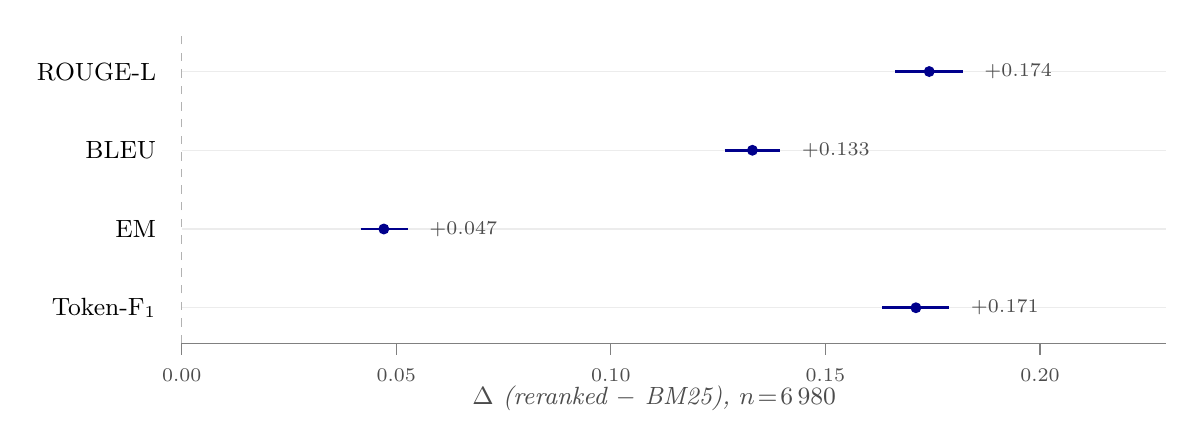
\begin{tikzpicture}[
    every node/.style={font=\small},
    point/.style={fill=blue!55!black, circle, inner sep=1.4pt},
    bar/.style={blue!55!black, line width=1pt},
  ]
    % Plot scale: value 0..0.22 maps to 0..12cm; \sx = 12/0.22 ~= 54.5
    \def\sx{54.5}

    % Y rows (top to bottom): ROUGE-L (4), BLEU (3), EM (2), Token-F1 (1)
    % Faint horizontal guide rules
    \foreach \y in {1,2,3,4} {
      \draw[gray!15, line width=0.4pt] (0,\y) -- (12.5,\y);
    }

    % Vertical zero reference
    \draw[dashed, gray!60] (0, 0.55) -- (0, 4.55);

    % X-axis ticks
    \draw[gray] (0, 0.55) -- (12.5, 0.55);
    \foreach \v in {0.00, 0.05, 0.10, 0.15, 0.20} {
      \pgfmathsetmacro{\xx}{\v * \sx}
      \draw[gray] (\xx, 0.55) -- (\xx, 0.40);
      \node[below=0.5mm, font=\scriptsize, gray!60!black]
        at (\xx, 0.40) {\v};
    }
    \node[font=\small\itshape, gray!60!black] at (6.0, -0.15)
      {$\Delta$ (reranked $-$ \bmtwofive{}),  $n\!=\!\fdev{}$};

    % --- ROUGE-L: 0.1742, [0.1663, 0.1820]
    \node[anchor=east, font=\small] at (-0.2, 4) {\rougel{}};
    \draw[bar] (0.1663*\sx, 4) -- (0.1820*\sx, 4);
    \node[point] at (0.1742*\sx, 4) {};
    \node[anchor=west, font=\scriptsize, gray!60!black]
      at (0.1820*\sx + 0.15, 4) {$+0.174$};

    % --- BLEU (sentence): 0.1330, [0.1265, 0.1395]
    \node[anchor=east, font=\small] at (-0.2, 3) {BLEU};
    \draw[bar] (0.1265*\sx, 3) -- (0.1395*\sx, 3);
    \node[point] at (0.1330*\sx, 3) {};
    \node[anchor=west, font=\scriptsize, gray!60!black]
      at (0.1395*\sx + 0.15, 3) {$+0.133$};

    % --- EM: 0.0471, [0.0417, 0.0527]
    \node[anchor=east, font=\small] at (-0.2, 2) {EM};
    \draw[bar] (0.0417*\sx, 2) -- (0.0527*\sx, 2);
    \node[point] at (0.0471*\sx, 2) {};
    \node[anchor=west, font=\scriptsize, gray!60!black]
      at (0.0527*\sx + 0.15, 2) {$+0.047$};

    % --- Token-F1: 0.1711, [0.1632, 0.1789]
    \node[anchor=east, font=\small] at (-0.2, 1) {Token-F$_1$};
    \draw[bar] (0.1632*\sx, 1) -- (0.1789*\sx, 1);
    \node[point] at (0.1711*\sx, 1) {};
    \node[anchor=west, font=\scriptsize, gray!60!black]
      at (0.1789*\sx + 0.15, 1) {$+0.171$};
  \end{tikzpicture}
  \caption{Headline paired-bootstrap forest plot
  (\Cref{tab:w3-ci}).  Dots: per-query mean $\Delta$ (reranked $-$
  \bmtwofive{}); bars: 95\,\% percentile interval, 10\,000 resamples,
  seed 42.  Dashed line at zero: all four intervals lie strictly
  above it, two-sided bootstrap $p\!<\!0.001$ throughout.}
  \label{fig:headline-forest}
\end{figure}

These CIs are $\sim\!6\times$ tighter than an earlier
200-query subsample comparison (n=200 vs.\ n=\fdev{}), and the
full-dev $\Delta$ point estimates all sit inside the 200-query CIs
--- so the original direction-and-magnitude claim survives the move
to full \devsmall{} intact, with the level numbers naturally
deflating to the harder full benchmark.

\paragraph{Retrieval-flag mechanism.}  The structural mechanism is
visible in a single retrieval flag: the rate of having $\geq\!1$
relevance-judged passage in the generator's top-3 jumps from
$\mathbf{20.8\,\%}$ (\bmtwofive{}) to $\mathbf{96.9\,\%}$ (reranked)
over the \fdev{} paired queries.  The reranker's job is precisely
to put the right passage in the generator's prompt; once it does,
T5-small (which we will see in \Cref{sec:w7} is extracting almost
all of its content from the prompt) reflects that.

\paragraph{Per-query outcome distribution.}  Per-query \Tokenf{}
splits 4\,015 strict improvements / 1\,766 regressions / 1\,199
ties --- i.e.\ a \emph{net} $+2\,249$ / \fdev{} queries
($\approx\!32\,\%$) strictly improved by feeding reranked passages,
with the regressions mostly clustered around already-easy queries
where \bmtwofive{} happened to surface a usable passage.  Of those
1\,766 strict per-query regressions, \textbf{233} fall into the
narrower \emph{regression bucket} on which \Cref{sec:w6} runs its
failure taxonomy: queries where the reranker actually brought the
relevant passage into the top-3 \emph{and} the generator's
\Tokenf{} dropped versus \bmtwofive{}.  The distinction matters
because the broader 1\,766 count contains retrieval-equivalent
queries on which the generator simply produced a different surface
form; the narrower 233 are the queries that ``should have'' worked
on retrieval grounds but didn't.

\paragraph{Bucket analysis by query type.}  \Cref{tab:bucket-by-type}
breaks the per-query \Tokenf{} $\Delta$ down by \msmarco{}
\texttt{query\_type}.

\begin{table}[H]
  \centering
  \caption{Paired \Tokenf{} broken down by \msmarco{}
  \texttt{query\_type}.  Same \fdev{} queries throughout.}
  \label{tab:bucket-by-type}
  \begin{tabular}{lrrrr}
    \toprule
    \texttt{query\_type} & $n$ & \bmtwofive{} & Reranked & $\Delta$ \\
    \midrule
    DESCRIPTION & 3\,725 & 0.1889 & 0.3939 & $\mathbf{+0.2050}$ \\
    ENTITY      &   631  & 0.1765 & 0.3186 & $+0.1421$ \\
    LOCATION    &   498  & 0.2495 & 0.3928 & $+0.1433$ \\
    NUMERIC     & 1\,665 & 0.1997 & 0.3235 & $+0.1238$ \\
    PERSON      &   461  & 0.2186 & 0.3557 & $+0.1371$ \\
    \bottomrule
  \end{tabular}
\end{table}

\texttt{DESCRIPTION} (53\,\% of the eval set) benefits most;
\texttt{NUMERIC} benefits least.  This direction is consistent with
the intuition that short numeric answers depend on lexical surface
match with the passage --- so semantic-aware reranking of nearly-
identical passages buys less than it does for long descriptive
answers where the right passage materially changes the available
phrasing.

\paragraph{Qualitative example.}  Query \texttt{1043064}
(\emph{``what is the chemical formula for oxygen tetrafluoride?''}).
\bmtwofive{} top-3 leads the generator to emit \emph{``Li\textsubscript{2}O''};
reranked top-3 leads it to emit \emph{``N\textsubscript{2}F\textsubscript{4}''}
--- the correct reference.  The retriever, not the generator,
changed.

\subsection{First-stage $\times$ reranker head-to-head}
\label{sec:w5a}

A natural follow-up to \Cref{sec:w5-dense-rerank}: does the same
cross-encoder recover \emph{more} from a weaker first stage?
\Cref{tab:w5a-results} runs the identical reranker over the
\bmtwofive{} top-100 (full 8.8M corpus) and over the dense
top-100 (50k sample), reporting absolute $\Delta$ and the
\emph{constrained recovery rate} $\Delta\,/\,(\recallH{} - \text{first-stage})$
that controls for each arm's recall ceiling.

\begin{table}[H]
  \centering
  \caption{Same cross-encoder applied to two first stages
  of very different starting strength.  ``Constrained recovery'' is
  $\Delta\,/\,(\recallH{} - \text{first-stage})$, which controls for
  the fact that a reranker can only re-order what the first stage
  returned into the top-100.  Same \fdev{} queries on both arms.}
  \label{tab:w5a-results}
  \small
  \setlength{\tabcolsep}{4pt}
  \begin{tabular}{@{}lrrrrr@{}}
    \toprule
    First stage           & \mrr{} (FS) & \mrr{} ($+$CE) & $\Delta_\mathrm{MRR}$ & Recov.\,\mrr{} & Recov.\,\ndcg{} \\
    \midrule
    \bmtwofive{} (8.8M)   & 0.1703      & 0.3554         & $+0.1851$             & 41.1\,\%        & 46.1\,\%        \\
    Dense L6 (50k)        & 0.8830      & 0.9304         & $+0.0474$             & 42.4\,\%        & 43.4\,\%        \\
    \bottomrule
  \end{tabular}
\end{table}

The absolute $\Delta$ favours the \bmtwofive{} arm by a factor of
nearly four (more room to recover), but the \emph{constrained
recovery rate} comes in essentially tied: $\sim\!42\,\%$ for MRR,
$\sim\!44\,\%$ for nDCG, on both arms.  The cleanest reading is
that the cross-encoder closes a fixed \emph{fraction} of the
ordering gap relative to the recall ceiling of its first stage,
regardless of whether that first stage is sparse or dense.

\paragraph{Caveat.}  The two arms are not on the same corpus: the
\bmtwofive{} arm runs on the full 8.8M-passage corpus, while the
dense arm runs on the 50k qrels-anchored sample
(\Cref{sec:w4-sampling-caveat}).  Absolute MRR levels are therefore
not comparable across arms, only the within-arm $\Delta$ and the
recovery rate.

\subsection{Evaluation layer}
\label{sec:w6}

\subsubsection{Semantic-proxy \bertscore{}}
\label{sec:w6-bertscore}

The four surface-form metrics in \Cref{tab:w3-ci} are all overlap-
or n-gram-based; T5-small's tendency to emit verbose extractive
outputs is a known source of mis-credit for surface-form
metrics~\cite{lin2004rouge,papineni2002bleu}.  The load-bearing
question of the evaluation layer is therefore: does the rerank $\Delta$ also show up
in a \emph{semantic} similarity scorer?

\Cref{tab:w6-bertscore} reports the DistilBERT-based \bertscore{}
proxy on a 3\,000-pair subsample of the shared qid set, with the
same paired-bootstrap-CI machinery as \Cref{tab:w3-ci}.

\begin{table}[H]
  \centering
  \caption{DistilBERT \bertscore{} proxy~\cite{zhang2020bertscore,sanh2019distilbert}
  on a 3\,000-pair subsample of the \fdev{} shared qid set.
  \texttt{rescale\_with\_baseline=True}, multi-reference max-$F_1$,
  paired bootstrap 10\,000 resamples seed 42, 95\,\% percentile
  interval.  Per-query: rerank strictly better 64.8\,\%, tie
  5.7\,\%, \bmtwofive{} strictly better 29.5\,\%.}
  \label{tab:w6-bertscore}
  \begin{tabular}{lrrrrr}
    \toprule
    Metric                       & \bmtwofive{} & Rerank & $\Delta$ & 95\,\% CI on $\Delta$ & $p$ (two-sided) \\
    \midrule
    \bertscore{}-$F_1$ (proxy)   & 0.2192       & 0.3920 & $\mathbf{+0.1728}$ & $[+0.1608,\,+0.1850]$ & $<0.001$ \\
    \bottomrule
  \end{tabular}
\end{table}

The semantic-proxy $\Delta$ ($+0.1728$) lands within $\pm 0.002$ of
the surface-form \Tokenf{} $\Delta$ ($+0.1711$) and the \rougel{}
$\Delta$ ($+0.1742$).  \textbf{The rerank gain is therefore not a
surface-form artefact.}  This is the result that justifies acting on
the surface-form CIs of \Cref{tab:w3-ci} without first running the
canonical \texttt{roberta-large} \bertscore{}.  The
\texttt{roberta-large} pass on full dev is reserved as a paper-
writing follow-up (citation-grade scorer, $\sim\!$hours of CPU); it
will refine the absolute level number but is not expected to change
the qualitative direction.

\subsubsection{Regression failure taxonomy}
\label{sec:w6-taxonomy}

\Cref{tab:w6-taxonomy} reports the 40-query seeded triage of the
233-strong regression bucket (\Cref{sec:gen-x-retrieval}).

\begin{table}[H]
  \centering
  \caption{Regression failure taxonomy on a 40-query seeded
  sample (seed 42) of the 233-strong regression bucket.  Labels are
  a deterministic five-way rule cascade; first-match wins.
  \texttt{semantic\_mismatch} is the residual catch-all.}
  \label{tab:w6-taxonomy}
  \begin{tabular}{lrr}
    \toprule
    Failure mode                & Count & Share \\
    \midrule
    \texttt{truncation\_midword}      & 22 & 55.0\,\% \\
    \texttt{truncation\_short} ($\leq\!3$ tok) & 14 & 35.0\,\% \\
    \texttt{topic\_drift}             &  2 &  5.0\,\% \\
    \texttt{extractive\_passage\_bias} & 2 &  5.0\,\% \\
    \texttt{semantic\_mismatch}       &  0 &  0.0\,\% \\
    \bottomrule
  \end{tabular}
\end{table}

$\mathbf{90\,\%}$ of the sample is generator-side truncation, not
retrieval or semantic failure.  Example (qid 49802,
\emph{``belizean cuisine''}): \bmtwofive{} produced a 24-token
descriptive paragraph; the reranked-arm prediction was the two
tokens \emph{``Belizean cuisine''} --- a passage title.  The
reranker is doing its job (richer passages); the generator's
extractive behaviour turns the richer context into less overlap-
matching output on this slice of queries.

At the time of the evaluation-layer report this observation pointed at the
\texttt{max\_new\_tokens=64} cap as the cheapest intervention.  The
closure run of \Cref{sec:w6-closure} \emph{falsifies} that reading.

\subsubsection{Decoding-budget closure: \texttt{mnt=64 $\to$ 128}}
\label{sec:w6-closure}

Same generator, same prompts, same retrieval inputs, same seed; the
\texttt{max\_new\_tokens} cap is the only thing that changes
(64 $\to$ 128).  \Cref{tab:w6-closure} reports the relevant signals.

\begin{table}[H]
  \centering
  \caption{Decoding-budget closure --- same paired generation comparison
  re-run with \texttt{max\_new\_tokens}~=~128.  Compared to the
  canonical \texttt{mnt=64} run on the same data.  None of the four
  surface-form deltas move by more than $0.005$; the regression
  bucket shrinks by 2 queries; the 40-query truncation share moves
  $2.5$~p.p.}
  \label{tab:w6-closure}
  \begin{tabular}{lrr}
    \toprule
    Signal                              & \texttt{mnt}~=~64 & \texttt{mnt}~=~128 \\
    \midrule
    \Tokenf{} $\Delta$                  & $+0.1711$ & $+0.1706$ \\
    \rougel{} $\Delta$                  & $+0.1742$ & $+0.1736$ \\
    BLEU $\Delta$                       & $+0.1330$ & $+0.1325$ \\
    EM $\Delta$                         & $+0.0471$ & $+0.0471$ \\
    Regression bucket size              & 233       & 231       \\
    Truncation share (40-query triage)  & 90.0\,\%  & 87.5\,\%  \\
    \bottomrule
  \end{tabular}
\end{table}

\textbf{The budget-cap hypothesis is falsified.}  T5-small is
hitting end-of-sequence \emph{naturally} on this prompt format;
the mid-word-ending output style observed in
\Cref{sec:w6-taxonomy} is intrinsic to the model on this prompt
shape, not a symptom of the 64-token cap.  Generator-side follow-up
work therefore has to target either prompt format (multi-passage
synthesis, citation-aware decoding) or the model itself
(T5-base or larger, instruction-tuned variants), not the
\texttt{max\_new\_tokens} knob.

\subsubsection{Question-form breakdowns}
\label{sec:w6-followups}

Three offline analyses on the per-query metrics; no new generation
or reranking required.

\paragraph{Question-form tagging.}  A nine-way syntactic
tagger over all \fdev{} \devsmall{} queries (who / what / when /
where / why / how / which / yes\_no / other).  Complementary to the
\msmarco{} native \texttt{query\_type} label of
\Cref{tab:bucket-by-type}: the two are correlated but not
redundant (e.g.\ ``who'' selects exclusively for \texttt{PERSON};
``where'' selects almost exclusively for \texttt{LOCATION}; ``what''
spans every \texttt{query\_type}).

\paragraph{Rerank $\Delta$ by question-form.}
\Cref{tab:w6b} reports per-form $\Delta$ \Tokenf{} with
paired-bootstrap CIs.

\begin{table}[H]
  \centering
  \caption{Rerank $\Delta$ \Tokenf{} by question-form on
  the full \fdev{} shared qid set, with paired-bootstrap 95\,\% CI
  (10\,000 resamples, seed 42).}
  \label{tab:w6b}
  \begin{tabular}{lrrr}
    \toprule
    Form    & $n$  & $\Delta$ \Tokenf{} & 95\,\% CI \\
    \midrule
    who     &  273 & $+0.1472$ & $[+0.1059,\,+0.1886]$ \\
    what    & 2\,751 & $+0.2097$ & $[+0.1964,\,+0.2232]$ \\
    when    &  189 & $+0.1207$ & $[+0.0813,\,+0.1590]$ \\
    where   &  283 & $+0.1774$ & $[+0.1427,\,+0.2157]$ \\
    why     &   75 & $+0.2267$ & $[+0.1509,\,+0.3082]$ \\
    how     &  837 & $+0.1520$ & $[+0.1321,\,+0.1737]$ \\
    which   &  120 & $+0.0250$ & $[-0.0281,\,+0.0773]$ \\
    yes\_no &  480 & $+0.0680$ & $[+0.0455,\,+0.0913]$ \\
    other   & 1\,972 & $+0.1643$ & $[+0.1497,\,+0.1801]$ \\
    \bottomrule
  \end{tabular}
\end{table}

\textbf{\texttt{which} (n=120) is the only question form whose
95\,\% CI on $\Delta$ \Tokenf{} includes zero} ($\Delta\!=\!+0.025$,
$p\!=\!0.33$), \emph{despite} a retrieval-side $\Delta$ \mrr{} of
$+0.71$ on the same subset.  Mechanism (hypothesised, not
confirmed): \texttt{which} queries are typically selection-style
(``which of X, Y, or Z is \ldots'') and require the generator to
choose among items the passage lists; reranking surfaces the right
passage but doesn't help the frozen extractive generator make the
selection.  The remaining factual wh-forms (what / where / why /
how / who) all see CIs strictly above zero in the $+0.12$ to
$+0.23$ range.

\paragraph{Structural profile of regression queries.}
Mann--Whitney U~\cite{mannwhitney1947} on five structural features
between the 233-query regression bucket and the 6\,747 non-regression
queries.  Four of the five features (query length in tokens,
query length in chars, number of qrels per query, \bmtwofive{}
top-3 average passage length) show no detectable difference at any
meaningful effect size.  The only signal: regression-arm top-3
passage lengths are marginally shorter
($\Delta\,\mathrm{median}\!=\!-2.7$ tokens, $p\!=\!0.0073$, rank-
biserial $r\!=\!-0.103$).  This is consistent with the
\Cref{sec:w6-taxonomy} truncation finding: shorter passages give
T5-small less material to extract.  See
\Cref{fig:w6c-query-length,fig:w6c-n-qrels,fig:w6c-top3-passage}.

\begin{figure}[H]
  \centering
  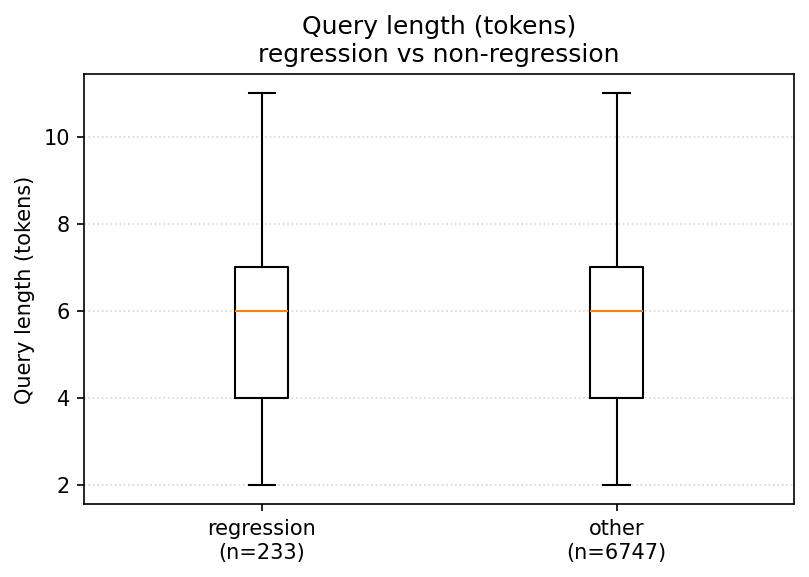
\includegraphics[width=0.62\linewidth]{figures/grounding_delta_vs_query_length.png}
  \caption{Query-length distribution, regression bucket
  (n=233) vs.\ rest (n=6\,747).  Indistinguishable; Mann--Whitney
  $p\!=\!0.96$, effect size $r\!=\!-0.002$.}
  \label{fig:w6c-query-length}
\end{figure}

\begin{figure}[H]
  \centering
  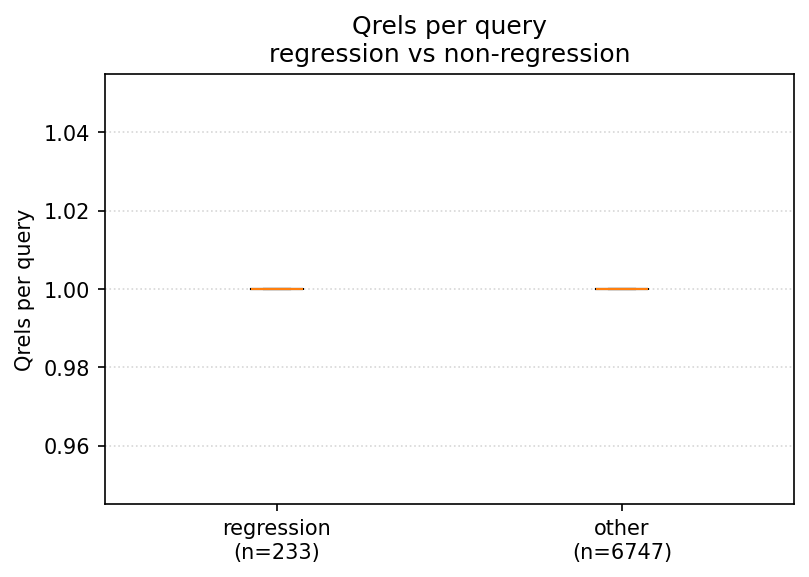
\includegraphics[width=0.62\linewidth]{figures/grounding_delta_vs_n_qrels.png}
  \caption{Number of relevance judgements per query.  A
  very small downward shift in the regression bucket
  ($p\!=\!0.009$, effect size $r\!=\!-0.040$); not meaningfully
  different from zero.}
  \label{fig:w6c-n-qrels}
\end{figure}

\begin{figure}[H]
  \centering
  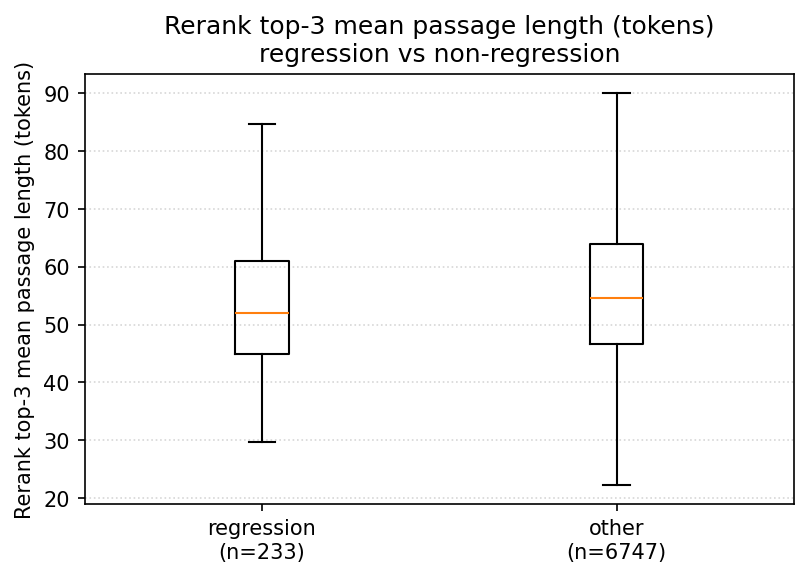
\includegraphics[width=0.62\linewidth]{figures/grounding_delta_vs_top3_passage_length.png}
  \caption{Average rerank top-3 passage length.  The only
  feature with a detectable effect: regression-arm top-3 passages
  are $\sim\!2.7$ tokens shorter at the median
  ($p\!=\!0.0073$, $r\!=\!-0.103$).  Consistent with
  \Cref{tab:w6-taxonomy}: shorter passages give T5-small less to
  extract.}
  \label{fig:w6c-top3-passage}
\end{figure}

\subsection{Grounding audit}
\label{sec:w7}

The evaluation-layer closure (\Cref{sec:w6-closure}) ruled out the decode budget
as the bottleneck.  The grounding audit answers the question the closure left open:
\emph{what is T5-small actually doing on this prompt format ---
extracting from the passages, or generating from parametric
memory?}

\subsubsection{Lexical and 3-gram grounding}

\Cref{tab:w7-lex-ngram} reports both lexical and 3-gram grounding
on the full \fdev{} paired qid set.

\begin{table}[H]
  \centering
  \caption{Lexical and 3-gram grounding on the full \fdev{}
  paired qid set.  Paired bootstrap 10\,000 resamples, seed 42,
  95\,\% percentile interval.  Both arms sit at the ceiling.}
  \label{tab:w7-lex-ngram}
  \begin{tabular}{lrrrrr}
    \toprule
    Metric             & \bmtwofive{} & Rerank & $\Delta$ & 95\,\% CI & $p$ \\
    \midrule
    Lexical content-token & 0.9972 & 0.9977 & $+0.0005$ & $[-0.0003,\,+0.0014]$ & $0.24$ \\
    3-gram                & 0.9873 & 0.9905 & $+0.0032$ & $[+0.0015,\,+0.0050]$ & $<\!0.001$ \\
    \bottomrule
  \end{tabular}
\end{table}

\textbf{Both arms sit at the ceiling.}  Almost every content word
T5-small emits is already in the prompt.  3-gram grounding is
slightly higher on the reranked arm
(reranking surfaces passages with phrasings closer to the gold
answer), but the $\Delta$ is $+0.003$ in absolute terms and both
arms remain $\sim\!99\,\%$.

\paragraph{Implication.}  T5-small on the
\texttt{question:\ \ldots\ context:\ \ldots} prompt is performing
\emph{extractive} QA, not generative QA.  The generation surface-form
$\Delta$ of \Cref{tab:w3-headline} is therefore almost entirely
\emph{downstream of retrieval}: the reranker puts the right words
into the prompt and the generator copies them.  This is a
\emph{calibration} of the headline result rather than a
contradiction --- the surface-form $\Delta$s are real, but the
mechanism is ``better passages\barrow{}better extractive output'',
not ``better passages\barrow{}better neural reasoning''.

\paragraph{Edge cases (reported separately).}  $\sim\!10\,\%$ of
predictions per arm are $<\!3$ tokens (the \texttt{truncation\_short}
/ \texttt{extractive\_passage\_bias} pattern from
\Cref{sec:w6-taxonomy}), scoring 3-gram grounding as $1.0$
vacuously.  Lexical-vacuous predictions are negligible
($<\!0.3\,\%$).  Counts are identical-shape on both arms, so the
paired $\Delta$ is unaffected.

\subsubsection{NLI-entailment grounding}
\label{sec:w7-nli}

\Cref{tab:w7-nli} reports an NLI-entailment proxy
($\text{entailment}(\text{passages} \to \text{prediction})$,
\code{cross-\allowbreak encoder/\allowbreak nli-\allowbreak deberta-v3-small}~\cite{he2023debertav3,williams2018mnli})
on the same 3\,000-paired-qid subsample as the \bertscore{}
proxy.

\begin{table}[H]
  \centering
  \caption{NLI-entailment grounding on the same 3\,000-
  paired-qid subsample (seed 42) used by the \bertscore{} proxy.
  Same paired-bootstrap CI convention.  This is the only paired
  metric in the entire project whose $\Delta$ reverses sign relative
  to the generation, reranking, and evaluation-layer surface-form story.}
  \label{tab:w7-nli}
  \begin{tabular}{lrrrrr}
    \toprule
    Metric    & \bmtwofive{} & Rerank & $\Delta$ & 95\,\% CI on $\Delta$ & $p$ \\
    \midrule
    NLI grounding & 0.2270   & 0.0821 & $\mathbf{-0.1448}$ & $[-0.1597,\,-0.1297]$ & $<\!0.001$ \\
    \bottomrule
  \end{tabular}
\end{table}

The NLI $\Delta$ is negative and strictly excludes zero.  Section
\Cref{sec:discussion-nli-flip} discusses the most plausible
mechanism and how to disambiguate.

\subsubsection{Grounding $\leftrightarrow$ downstream
correlation}

Per-query Spearman / Pearson correlations between each grounding
metric and downstream \Tokenf{} / \bertscore{}-$F_1$, with the
high-vs-low ($\geq\!0.9$) bin Mann--Whitney as a second cut.

\textbf{Direction is uniformly positive but magnitudes are small.}
Every binned cell has high-grounding $-$ low-grounding $>\!0$;
absolute differences sit between $0.04$ and $0.10$ on the
\Tokenf{} / \bertscore{} scale.  Per-query Spearman / Pearson
correlations are near zero (\textbar$\rho$\textbar~$<\!0.05$ in
every cell), entirely because both arms sit at the lex / 3-gram
ceiling on $\geq\!99\,\%$ of queries.  The signal is in the
\emph{level}, not the per-query rank.

\subsubsection{Low-grounding case study}

Of the 197 rerank-arm queries with $\mathrm{lex}\!<\!0.9$ OR
$\mathrm{ngram}\!<\!0.9$, 30 are sampled (seed 42) and labelled by
a coarse five-way rule cascade.  \Cref{tab:w7d} reports the
counts.

\begin{table}[H]
  \centering
  \caption{Low-grounding case study on a 30-query seeded
  triage (seed 42) of the 197 rerank-arm queries with
  lex $<\!0.9$ or 3-gram $<\!0.9$.  Categories applied in
  declaration order; first match wins.
  \texttt{parametric\_or\_external} would flag genuine
  hallucinations.}
  \label{tab:w7d}
  \begin{tabular}{lrr}
    \toprule
    Label                       & Count & Share \\
    \midrule
    \texttt{paraphrase\_reorder}     & 23 & 77\,\% \\
    \texttt{partial\_external}       &  7 & 23\,\% \\
    \texttt{parametric\_or\_external} & 0 &  0\,\% \\
    \texttt{prediction\_too\_short}  &  0 &  0\,\% \\
    \texttt{residual}                &  0 &  0\,\% \\
    \bottomrule
  \end{tabular}
\end{table}

The 23 \texttt{paraphrase\_reorder} cases have all the content
words in the prompt; only the order or phrasing changes.  The 7
\texttt{partial\_external} cases are almost entirely
tokenisation / morphology artefacts: \emph{``350oF''} vs.\
\emph{``350$^\circ$F''}, \emph{``competed''} vs.\ \emph{``compete''}.
\textbf{Zero genuine hallucinations} (\texttt{parametric\_or\_external})
in the sample.  This reinforces the grounding-audit headline: T5-small on this
prompt format is doing extractive QA even on its worst-grounded
outputs.

\subsection{RAG triad diagnostic interface}
\label{sec:w8-triad}

The current repository adds a deterministic triad report as an
engineering-facing diagnostic layer over the same generation prediction
schema.  The \texttt{mgq-rag-triad} CLI writes
\texttt{metrics.json}, \texttt{per\_query\_triad.jsonl},
\texttt{low\_score\_cases.jsonl}, and \texttt{report.md} for one or
more generation configurations.  The three dimensions are kept
separate: context relevance (qrels hit when qrels are supplied,
otherwise query--context lexical overlap), groundedness (lexical
content-token support in the shown passages), and answer relevance
(\Tokenf{} against the stored reference answers).

This is intentionally not promoted to a new headline result in this
report.  Its role is to make future regressions easier to diagnose:
a low triad row can be inspected as retrieval-side evidence failure,
unsupported generation, answer mismatch, or a combination of those
failure modes.  The CLI rejects unsupported evaluator names, so
future model-assisted RAGAS/TruLens-style scoring must be opted into
explicitly rather than silently mixed with deterministic scores.

\subsection{Context packing and prompt compression}
\label{sec:w9-context-packing}

The current repository also adds a deterministic context-packing
layer for generation runs.  It is disabled for the historical
baselines, but can be enabled with \texttt{mgq-generate
--context-packing}.  The packer uses character budgets as a
CPU-friendly proxy for token cost, supports per-passage trimming,
query-overlap sentence selection, deduplication, and rank-preserving
ordering, and records span metadata that maps the packed prompt
context back to source document ids.

The paired report is produced by
\texttt{mgq-context-packing-report}.  It compares an uncompressed
\texttt{predictions.jsonl} file against a compressed one on matched
query ids, then writes \texttt{comparison.json},
\texttt{per\_query.jsonl}, and \texttt{report.md}.  The report keeps
answer-quality deltas (\Tokenf{} and exact match) separate from
context-character savings, so compression can be evaluated as a
cost--quality trade-off rather than as a hidden prompt-format change.
Grounding and triad reports should be read alongside this output
before treating a packed prompt as a better RAG configuration.

% =============================================================================
\clearpage\section{Discussion}
\label{sec:discussion}

\subsection{Where does the rerank gain come from?}
\label{sec:discussion-where}

Combining \Cref{sec:gen-x-retrieval} with \Cref{sec:w7}, the answer
is unambiguous: the headline doubling of generation surface-form metrics is
\textbf{a retrieval effect, not a generation effect}.  T5-small on
this prompt format does not invent content; it copies content from
the prompt.  The reranker's job is to ensure that the content the
generator copies is the \emph{right} content.  Two pieces of
evidence converge:

\begin{enumerate}
  \item The retrieval-flag rate of having $\geq\!1$
        relevance-judged passage in the top-3 jumps from 20.8\,\%
        to 96.9\,\% across the two arms (\Cref{sec:gen-x-retrieval}).
        This is the proximate mechanism.
  \item Lexical content-token grounding sits at $\sim\!0.997$ on
        both arms (\Cref{tab:w7-lex-ngram}).  Whatever content
        words T5-small emits, $\sim\!99.7\,\%$ of them are already
        in the prompt.  There is no slack for ``the generator
        thought of something better'' to account for any meaningful
        portion of the generation $\Delta$.
\end{enumerate}

This reading has direct consequences for where further work should
go.  Decoding-budget interventions are ruled out by
\Cref{sec:w6-closure}; generator output-style interventions
(\Cref{sec:w7-nli}) are constrained by the ceiling effect; prompt-
format and generator-capacity interventions become the natural next
axes.  \Cref{sec:plan-vs-actual} records the generator-capacity (T5-base swap)
follow-up that is queued in the project's reduced-scope plan.

\subsection{The NLI sign flip}
\label{sec:discussion-nli-flip}

\Cref{tab:w7-nli} is the only paired metric in this project whose
$\Delta$ reverses sign relative to the otherwise-consistent generation,
reranking, and evaluation-layer
story: a robust $-0.145$, with a 95\,\% CI that strictly excludes
zero.  Three candidate explanations are worth taking seriously.

\paragraph{(i) Output-shape artefact (currently the best-supported).}
The 40-query taxonomy (\Cref{tab:w6-taxonomy}) and the low-grounding case
study (\Cref{tab:w7d}) jointly show that the reranked-arm
predictions contain more fragmentary / mid-word-cut / title-style
outputs than the \bmtwofive{}-arm predictions.  A sentence-level
NLI cross-encoder cannot \emph{entail} a fragmentary hypothesis ---
it requires syntactically complete propositions on both sides.  So
even when the rerank-arm prediction is lexically faithful (it
copies content tokens from the right passage), the NLI scorer
correctly returns low entailment because the prediction \emph{as
a sentence} is incomplete.  Under this account, the NLI flip is a
metric--model mismatch on a particular output style, not a
semantic regression.

\paragraph{(ii) True semantic regression on some slice.}  It is
also possible that the reranker, by surfacing tighter / more on-
topic passages, paradoxically encourages T5-small to extract
title-style or list-style fragments instead of the descriptive
paragraphs that would actually be reference-equivalent.  Under this
account the NLI flip is real: rerank-arm predictions are, on a
semantic-faithfulness scale, worse despite being lexically tighter.
This is harder to rule out from the existing data because the grounding
binned analysis shows a small positive correlation between
grounding and downstream metrics (\Cref{sec:w7}), but the
sentence-completeness confound is unresolved.

\paragraph{(iii) NLI checkpoint artefact.}  The NLI cross-encoder
in the NLI-grounding audit is \texttt{\seqsplit{cross-encoder/nli-deberta-v3-small}} ---
distilled, MNLI-trained~\cite{he2023debertav3,williams2018mnli}.
It is not domain-adapted to \msmarco{}-style passages and could
behave differently from a larger NLI scorer on the project's
characteristic short-passage / short-prediction inputs.

\paragraph{How to disambiguate.}  The cleanest test is a generator
swap: rerun the paired generation comparison with T5-base (or an
instruction-tuned small model) in place of T5-small, holding
everything else fixed, and recompute the NLI proxy.  If the NLI
$\Delta$ moves toward zero or flips back positive without changing
the surface-form $\Delta$ much, account~(i) is supported.  If it
stays negative at the same magnitude, account~(ii) becomes the
working hypothesis.  This is the planned generator-capacity follow-up, deferred
to the post-deadline T5-base run (\Cref{sec:plan-vs-actual}).

\subsection{Plan vs.\ actual}
\label{sec:plan-vs-actual}

The project's initial 12-stage plan named the milestones in
\Cref{tab:plan-vs-actual}.  Eleven milestones elapsed; the
table records what shipped, what was substituted, and what was
de-scoped.

\small
\begin{longtable}{@{}
    p{1.10cm}
    >{\raggedright\arraybackslash}p{3.70cm}
    >{\raggedright\arraybackslash}p{7.35cm}
    >{\raggedright\arraybackslash}p{2.10cm}@{}}
\toprule
\textbf{Stage} & \textbf{Plan} & \textbf{Actual} & \textbf{Status} \\
\midrule
\endfirsthead
\toprule
\textbf{Stage} & \textbf{Plan} & \textbf{Actual} & \textbf{Status} \\
\midrule
\endhead
Stage 1 & EDA & EDA on the QA v2.1 validation 5k-row sample
     (\Cref{sec:dataset}) & shipped \\
Stage 2 & \bmtwofive{} baseline & Full 8.8M-corpus \bmtwofive{} retrieve
     +  MRR/Recall (\Cref{sec:w2-results}) & shipped \\
Stage 3 & RAG baseline (T5/BART/Phi + top-3) & T5-small RAG generator on
     the BM25 top-3, 200-query sample baseline + the load-bearing
     paired full-dev comparison (\Cref{sec:gen-x-retrieval}) & shipped \\
Stage 4 & Dense retrieval, ideally ANCE & Generic \texttt{all-MiniLM-L6-v2}
     on a 50k qrels-anchored sample with FAISS \texttt{IndexFlatIP}
     (\Cref{sec:w4-results}); same-tier encoder horizontal added
     (\Cref{sec:w4b}: MiniLM-L12, bge-small-en-v1.5; bge-small wins
     $+0.019$ \mrr{}) and density-sensitivity sweep added
     (\Cref{sec:w4a}: 15k/30k/50k samples).  ANCE /
     \msmarco{}-tuned encoders and true low-density cells
     (1/5/10\,\%, needing 70k--700k samples) deferred & shipped \\
Stage 5 & Cross-encoder rerank & \texttt{ms-marco-MiniLM-L-6-v2} over
     dense top-100, full-dev (\Cref{sec:w5-dense-rerank}) +
     \bmtwofive{}-top-100 arm (\Cref{sec:w5a}) & shipped \\
Stage 6 & Generator fine-tuning & \emph{Substituted}: evaluation layer
     (\bertscore{} proxy + failure taxonomy + decode-budget closure;
     \Cref{sec:w6}).  The paired generation comparison made evaluation
     calibration the higher-leverage axis than SFT, and the evaluation-layer
     closure + grounding together explain why SFT is unlikely
     to be the bottleneck. & substituted \\
Stage 7 & Hallucination \& citation & \emph{Substituted}: grounding audit
     (lexical / 3-gram / NLI; \Cref{sec:w7}).  Same goal
     (faithfulness), more direct measurement.  Span-level citation
     linking is in the explicit out-of-scope list. & substituted \\
Stage 8 & Long-document handling & \emph{De-scoped} due to the project's
     2026-05-22 deadline and the choice to prioritise the evaluation and grounding
     analyses on the already-shipped passage-level pipeline.
     The infrastructure (sliding-window prompt assembly) exists in
     the runner; the long-doc benchmark pass does not. & de-scoped \\
Stage 9 & Integration \& acceleration (ONNX, quantisation) & Engineering
     scaffolding shipped (manifests, lockfile, CI, lint;
     \Cref{sec:reproducibility}); ONNX / quantisation
     not pursued on the CPU-only laptop where wall-clock cost is
     already dominated by the cross-encoder. & partial \\
Stage 10 & Final evaluation & The headline paired comparison serves as
     the final evaluation; no CodaLab submission. & redirected \\
Stage 11 & Research paper & This report. & shipped \\
Stage 12 & Presentation & Out of report scope. & --- \\
\bottomrule
\caption{Plan vs.\ actual.  ``Substituted'' indicates that the
planned milestone was replaced by an evidence-driven alternative
that addressed the same underlying goal; ``de-scoped'' indicates
work that was cut, not redirected.}
\label{tab:plan-vs-actual} \\
\end{longtable}
\normalsize

The two evaluation and grounding substitutions are the project's main methodological
deviation from the plan.  The reasoning was empirical: once the paired generation
comparison shipped, evaluation calibration --- ``do these
deltas hold up under a semantic-similarity scorer?'', ``where do
the remaining regressions come from?'' --- gave a clearer story
than SFT would have, and the evaluation-layer closure run then made that story
\emph{actionable} by ruling out the most plausible cheap
intervention (the decoding budget).  The grounding audit then
calibrated the headline result honestly: most of the gain is
retrieval, the generator is extractive, and the only sign-
reversing metric (\Cref{sec:w7-nli}) is plausibly an output-shape
artefact that a generator swap could disambiguate.

% =============================================================================
\clearpage\section{Limitations}
\label{sec:limitations}

\paragraph{No fine-tuning anywhere.}  No SFT pass on
$(\text{question}, \text{gold passage}, \text{answer})$ triples has
been run.  Every model is used as a generic pretrained checkpoint:
T5-small for generation, \texttt{all-MiniLM-L6-v2} for dense
retrieval, \texttt{ms-marco-MiniLM-L-6-v2} for the cross-encoder
(\msmarco{}-trained, but as-is).  The absolute level numbers
(\rougel{}~$\approx\!0.18$ on \bmtwofive{}, $\approx\!0.36$ on
reranked) are therefore modest; the load-bearing claim is the
paired $\Delta$ between rows, which is statistically robust on
$n\!=\!\fdev{}$.

\paragraph{Dense and rerank numbers are on a qrels-anchored sample.}  The dense
50k sample includes every \devsmall{} relevant doc by construction
(\Cref{sec:w4-sampling-caveat}), inflating absolute MRR / Recall
on the sampled setting.  The legitimate comparison is within-
sample (dense vs.\ \bmtwofive{} on the same pool), not against the
full-corpus number.  This caveat is propagated to the dense+
rerank numbers, which inherit the same sampling.

\paragraph{TREC-DL is retrieval evidence, not generation evidence.}
The full-corpus 2019/2020 benchmark in
\Cref{sec:trec-dl-results} establishes that MiniLM reranking improves
local ordering under deep graded judgments.  It does not evaluate the
generator, prove cross-domain RAG generalization, or remove the
candidate-recall ceiling.  The top-100 reranked files also cannot
support a paired Recall@1000 claim; that value is reported only for
the top-1,000 \bmtwofive{} first stage.

\paragraph{BEIR transfer is narrow retrieval evidence.}
The NFCorpus and SciFact results in \Cref{sec:beir-results} use their
own non-MS-MARCO corpora and show a consistent early-ranking lift from
the unchanged reranker.  They cover only two relatively small retrieval
collections and do not evaluate generation or grounded answers.  They
therefore support transfer on these collections, not broad cross-domain
RAG generalization.

\paragraph{The SciFact first-stage diagnosis is quantitative only.}
\Cref{sec:scifact-first-stage} shows that the SciFact top-100
candidate set is much less restrictive than NFCorpus under the frozen
\bmtwofive{} run, but it does not explain every residual miss.  The
24 depth-recoverable and 11 top-1,000-miss queries still require
case-level inspection before attributing them to vocabulary mismatch,
claim wording, qrels coverage, or model capacity.

\paragraph{The NFCorpus query-representation result is subset-specific.}
The comparison in \Cref{sec:nfcorpus-first-stage} uses the official
102-query video subset because bounded source descriptions can be
recovered and frozen for that cohort.  It does not cover the remaining
221 test queries.  The descriptions are source-page context related to
how NFCorpus judgments were constructed, not independent user queries;
the observed gain therefore supports a benchmark-representation
diagnosis, not general query-expansion effectiveness.  The 72-case
taxonomy is also a single-reviewer descriptive census without
inter-annotator agreement.

\paragraph{\bmtwofive{} tokenizer mismatch with Anserini.}  The full-corpus
\mrr{}~$=0.170$ versus reference $\approx 0.184$ is mostly
attributable to tokenizer differences between \texttt{bm25s} default
and Lucene \texttt{EnglishAnalyzer}.  Acceptable for a single-
machine pure-Python pipeline, but it does mean the project's
\bmtwofive{} number cannot be directly compared to published
Lucene-tokenizer baselines without bracketing for the tokenizer gap.

\paragraph{Generation metrics are dominated by surface form.}  The
\bertscore{} proxy (\Cref{sec:w6-bertscore}) and the
grounding metrics (\Cref{sec:w7}) partially close the surface-form
gap, but the canonical \texttt{roberta-large} \bertscore{} on full
dev/small is still open.

\paragraph{The NLI sign flip is unresolved.}
\Cref{sec:discussion-nli-flip} identifies three candidate
mechanisms; existing data cannot fully discriminate among them.
A T5-base / instruction-tuned-small generator swap is the
disambiguating experiment.

\paragraph{\devsmall{} only, single seed for the distractor sample.}
No held-out test split.  The distractor sample is deterministic
(seed 42) but not averaged across multiple seeds.

\paragraph{CPU-only execution across two machines.}  The core MS~MARCO
experiments were produced on a six-core Apple Silicon laptop.  The
July 2026 TREC-DL and BEIR retrieval benchmarks were run on Windows
with CPU-only PyTorch.  That Windows machine contains an NVIDIA GPU,
but the recorded environments did not use it.  The single-machine,
CPU-execution constraint keeps each stage reproducible, but it caps the
kinds of generators that can be evaluated within the deadline.

% =============================================================================
\clearpage\section{Conclusion}
\label{sec:conclusion}

The principal empirical claim of this report is the following.
On \msmarco{} Passage \devsmall{} (\fdev{} queries), replacing
the upstream retriever from \bmtwofive{} with a cross-encoder-
reranked dense top-3 --- holding the generator, the prompt, and
the random seed fixed --- approximately doubles every
surface-form generation metric, with 95\,\% paired-bootstrap
confidence intervals strictly above zero on all four metrics
(\Cref{tab:w3-ci}).  The effect is corroborated by a
\bertscore{} semantic-similarity proxy at essentially the same
magnitude (\Cref{tab:w6-bertscore}).  However, the grounding
audit of \Cref{sec:w7} shows that both arms operate at the
$\sim\!99\,\%$ lexical and 3-gram grounding ceiling: under this
prompt format T5-small is performing extractive QA, and the
observed gain is almost entirely attributable to retrieval
rather than to generation.

The methodological contribution of the project lies in the
discipline of treating every cross-stage comparison as a paired
statistical test and of calibrating each surface-form metric
against a semantic-similarity proxy and a grounding metric before
accepting it as evidence.  Three readings that would have appeared
plausible from the generation surface-form numbers alone are rejected on
this basis: that the residual regression bucket is driven by the
decoding budget (falsified in \Cref{sec:w6-closure}), that
reranking materially improves grounding (\Cref{tab:w7-lex-ngram}
shows both arms at the lexical ceiling), and that the rerank
$\Delta$ is uniformly positive across metric families
(\Cref{tab:w7-nli} shows the NLI proxy reversing sign).

The external retrieval evidence adds a second, bounded conclusion.
The unchanged cross-encoder improves early ranking on TREC-DL 2019/2020
and on the BEIR NFCorpus and SciFact collections, while fixed
Recall@100 shows that reranking cannot repair missing candidates.  The
NFCorpus follow-up localises much of that ceiling to compact query
representation: on the 102-query video subset, adding the bounded
official description raises \recallH{} from 0.2821 to 0.3700 under the
same \bmtwofive{} system.  This does not supersede the main generation
result and does not establish cross-domain generation.  The matching
SciFact first-stage diagnosis is milder: most queries already have
complete relevant-document coverage at depth 100, so the large
NFCorpus ceiling should be treated as dataset- and representation-
sensitive rather than a general failure of the unchanged first stage.

The most informative follow-up experiment is a generator-capacity
swap (T5-base or an instruction-tuned small model) on the same
prompts and the same retrieval inputs.  Such an experiment
simultaneously tests whether the surface-form $\Delta$ extends
with capacity, whether the NLI sign flip persists under a more
verbose generator, and whether the lexical-grounding ceiling
moves.  Each outcome is independently informative for the design
of CPU-tractable open-domain QA pipelines on this benchmark.

\subsection*{Future work}
\label{sec:future-work}

The roadmap has become more explicit since the original experiment
window.  The next steps are grouped by what they test rather than by
stage number:

\begin{itemize}
  \item \textbf{TREC-DL reference expansion.}  The graded evaluator
        and full-corpus \bmtwofive{}+MiniLM reference are complete
        (\Cref{sec:trec-dl-results}).  The next valid comparison is a
        learned-sparse or late-interaction system under the same
        per-track qrels, candidate-depth, and independent-evaluator
         contract --- not an aggregate that hides the 2019/2020
         difference.
  \item \textbf{NFCorpus first-stage retrieval.}  The cross-domain
        benchmark in \Cref{sec:beir-results} shows that reranking helps
        once candidates are present, while the bounded source-context
        comparison in \Cref{sec:nfcorpus-first-stage} recovers part of
        the video-subset ceiling without changing \bmtwofive{}.  The
        remaining valid comparison is a separately predeclared hybrid,
        dense, or learned-sparse first stage on a frozen cohort and
        fixed depth; it should not be selected after inspecting the
        same queries or presented as part of the completed ablation.
  \item \textbf{Retrieval fusion and retrieval measurement.}
        Extend the current reciprocal-rank-fusion runner and
        same-qid matrix report with learned sparse retrieval as a
        SPLADE-style baseline, then report \mrr{} / \ndcg{}
        consistently across first-stage, reranked, and fused
        retrieval outputs.
  \item \textbf{Reranker alternatives.}  Evaluate BGE-style
        cross-encoder reranking and a ColBERT-style late-interaction
        path against the current MiniLM cross-encoder under matched
        candidate sets, including latency and memory notes.
  \item \textbf{Chunking and context assembly.}  Add semantic
        chunking and parent-child chunk retrieval experiments, then
        measure whether better context reconstruction improves the
        generation and grounding metrics without inflating prompt
        length.
  \item \textbf{Query transformation and adaptive retrieval.}
        Add query expansion/de-contextualisation before retrieval and
        a retrieval-sufficiency check after reranking.  The
        sufficiency layer should trigger a second retrieval pass or
        abstention rather than forcing unsupported generation.
  \item \textbf{Evaluation hardening.}  Extend the current paired
        bootstrap protocol and deterministic triad report with
        full-sample \texttt{roberta-large} \bertscore{}, an
        alternative-family faithfulness scorer, multiple-comparison
        correction.
  \item \textbf{Offline/online separation.}  Split batch indexing
        from online query handling: an offline job should read data,
        chunk passages, embed, build FAISS, and persist the index;
        the online path should load the index and serve retrieval or
        generation requests through a narrow API.
  \item \textbf{Generator and prompt ablations.}  Continue the
        T5-base / FLAN-T5 capacity sweep, citation-aware prompts, and
        tokenizer-aware prompt-compression work to test whether the
        current extractive-grounding ceiling can be moved without
        sacrificing faithfulness.
\end{itemize}

The reproducibility scaffold (\Cref{sec:reproducibility}) is
designed so that each follow-up adds a controlled configuration or
adapter, not a separate experimental codebase.

% =============================================================================
\clearpage
\section*{Acknowledgements}
\addcontentsline{toc}{section}{Acknowledgements}

The project depends entirely on open-source artefacts: \msmarco{}
itself~\cite{bajaj2016msmarco,nguyen2016msmarcoqa},
the Pyserini / Anserini ecosystem and the \texttt{bm25s}
re-implementation~\cite{lin2021pyserini,lu2024bm25s}, FAISS for
exact dense search~\cite{johnson2019faiss}, the Sentence-Transformers
and Hugging Face Transformers
ecosystems~\cite{reimers2019sbert,wolf2020transformers}, the
\texttt{ir\_datasets} loader~\cite{macavaney2021irdatasets}, the
T5 pretrained model~\cite{raffel2020t5}, the
\texttt{cross-encoder/ms-marco-MiniLM-L-6-v2} reranker, the
DistilBERT and DeBERTa~v3
encoders~\cite{sanh2019distilbert,he2023debertav3}, and the
\texttt{rouge\_score} / \texttt{sacrebleu} / \texttt{evaluate}
metric libraries~\cite{lin2004rouge,papineni2002bleu}.

\clearpage
% --- References --------------------------------------------------------------
\printbibliography[heading=bibintoc,title={References}]

% =============================================================================
\clearpage
\appendix

\section{Configuration and reproducibility}
\label{sec:reproducibility}

\subsection{One config, workflow facade, and stage runners}

All four modelling-stage runners are driven by a single configuration file
at \texttt{configs/baseline.yaml}; the evaluation and grounding analysis scripts and
the triad CLI read the on-disk paired generation predictions directly.  The current repository
also exposes a workflow facade through \texttt{rag-eval} and
installable \texttt{mgq-*} console scripts.  \Cref{tab:repro-cmds}
records the canonical command family for each layer.

\begin{table}[H]
  \centering\small
  \caption{One canonical command per stage.  All commands assume
  the project root as working directory and \texttt{pip install -e
  .} has registered the \texttt{src} package.}
  \label{tab:repro-cmds}
  \begin{tabularx}{\linewidth}{l>{\ttfamily\raggedright\arraybackslash}X}
    \toprule
    Stage & \normalfont Command \\
    \midrule
    Workflow facade & rag-eval run \mbox{--config} configs/baseline.yaml \mbox{--dry-run} \\
    Sparse retrieval  & python experiments/run\_retrieval.py \\
    TREC-DL \bmtwofive{} & mgq-retrieve \mbox{--dataset} \seqsplit{msmarco-passage/trec-dl-2019/judged} \mbox{--resume} {\normalfont (repeat for 2020)} \\
    TREC-DL reranking & mgq-rerank \mbox{--dataset} \seqsplit{msmarco-passage/trec-dl-2019/judged} \mbox{--resume} {\normalfont (repeat for 2020)} \\
    BEIR \bmtwofive{} & mgq-retrieve \mbox{--dataset} \seqsplit{beir/nfcorpus/test} \mbox{--resume} {\normalfont (repeat for SciFact)} \\
    BEIR reranking & mgq-rerank \mbox{--dataset} \seqsplit{beir/nfcorpus/test} \mbox{--resume} {\normalfont (repeat for SciFact)} \\
    NFCorpus first-stage diagnosis & make analyze-nfcorpus-first-stage \\
    SciFact first-stage diagnosis & make analyze-scifact-first-stage \\
    NFCorpus failure review & make review-nfcorpus-first-stage \\
    NFCorpus video exact-output reproduction & make reproduce-nfcorpus-video-eval \\
    Generation  & python experiments/run\_generation\_baseline.py \\
    Dense retrieval  & python experiments/run\_dense\_retrieval.py \\
    Reranking  & python experiments/run\_reranker.py \\
    Generation paired    & python scripts/run\_full\_generation\_and\_analysis.py \\
    First-stage head-to-head & python scripts/compare\_rerank\_first\_stages.py \\
    Evaluation BERTScore & python scripts/bertscore\_paired\_eval.py \\
    Evaluation taxonomy  & python scripts/regression\_failure\_taxonomy.py \\
    Evaluation closure   & python scripts/run\_full\_generation\_and\_analysis.py \mbox{--max-new-tokens}~128 \mbox{--out-suffix}~\_mnt128 \\
    Question-form breakdowns & scripts/tag\_query\_forms.py \ /\ analyze\_rerank\_by\_query\_form.py \ /\ regression\_query\_profile.py \\
    Grounding & python scripts/grounding\_audit.py \\
    NLI grounding     & same script with \mbox{--nli-n-pairs}~3000 \\
    Triad     & mgq-rag-triad \mbox{--predictions} bm25=\ldots{} \mbox{--predictions} reranked=\ldots{} \mbox{--output-dir} outputs/rag\_triad \\
    Context packing & mgq-context-packing-report \mbox{--baseline-predictions} \ldots{} \mbox{--compressed-predictions} \ldots{} \mbox{--output-dir} outputs/context\_packing \\
    Input validation & docs/input\_validation.md \\
    Model-stack smoke & python scripts/smoke\_model\_stack.py \mbox{--config} configs/baseline.yaml \mbox{--device} cpu \\
    Serving smoke & mgq-serve \quad{\normalfont(after installing the \texttt{serve} extra)} \\
    \bottomrule
  \end{tabularx}
\end{table}

\subsection{Manifests}

Every runner writes \texttt{outputs/<stage>/manifest.json} alongside
\texttt{metrics.json}.  The manifest records: the current git
commit (and a ``dirty'' flag if any tracked file was modified at
launch time), the command line, the configuration file SHA-256,
the requirements/lockfile/pyproject SHA-256s, and a per-output
SHA-256 (truncated) for every file the runner emits.  This is
sufficient to verify that a re-run produced byte-identical outputs,
or to identify exactly which input changed if the outputs differ.

\subsection{Input validation boundary}

The repository now distinguishes research-data assumptions from
production-facing inputs.  TREC \texttt{run.tsv} readers reject
malformed six-column rows, empty identifiers, invalid or duplicate
ranks, rank gaps, duplicate documents within a query, non-finite
scores, and non-UTF-8 bytes before expensive generation or analysis
starts.  The independent evaluation adapter additionally rejects
duplicate qrels judgments and ambiguous four-column layouts, and
writes rank-preserving canonical scores before invoking a standard
evaluator.
Generation prompt assembly normalises whitespace, rejects empty
queries, drops empty optional passages, and applies deterministic
character truncation before tokenizer-level truncation.  Serving
JSONL loaders reject duplicate ids, missing fields, invalid JSON,
replacement-character-heavy text, and non-object records.  The
FastAPI wrapper maps these typed validation failures to structured
\texttt{422} payloads with \texttt{error.type},
\texttt{error.message}, and \texttt{error.field}.

\subsection{Determinism}

Seed 42 is used everywhere a random choice enters: the dense
qrels-anchored distractor sample, the BERTScore subsample
selection, the regression-bucket triage sample, the
low-grounding case-study sample, and the 10\,000-resample paired
bootstrap throughout.  This is documented in the per-script CLI
help and in the per-stage reports' ``Reproduce'' sections.

\subsection{What is and isn't committed}

The project's local operating contract codifies the policy:
\texttt{outputs/}, \texttt{data/}, and the local-scratch directory
are gitignored.  The tracked artefacts are source code (under
\texttt{src/}, \texttt{experiments/}, \texttt{scripts/},
\texttt{tests/}), configs, documentation, compact report outputs
under \texttt{reports/}, and the figures required to render those
reports.  Large regenerable artefacts (every \texttt{metrics.json},
every \texttt{run.tsv}, every dataset cache, every model cache) stay
outside git.  Exact public ranked outputs needed to reproduce the
external benchmark tables are distributed separately as three
checksum-verified GitHub Release archives.  The same 14 TREC-format
runs, their manifests, checksums, and a normalized Parquet view are
mirrored in the public Hugging Face Dataset
\href{https://huggingface.co/datasets/GioiaZheng/msmarco-genqa-benchmark-runs}%
{\texttt{GioiaZheng/msmarco-genqa-benchmark-runs}}.  Neither surface
redistributes benchmark text, qrels, model weights, or local caches.

\subsection{Public report and artifact surfaces}

The repository remains the source of truth for code, contracts, and
human-readable result interpretation.  The current PDF and HTML report
are tracked under \texttt{reports/repo\_report/}.  Exact outputs are
available from the versioned GitHub Releases and the Hugging Face
Dataset above.  A concise project-facing summary is maintained at
\href{https://gioiazheng.github.io/projects/msmarco-genqa/}%
{\texttt{gioiazheng.github.io/projects/msmarco-genqa/}}.  These
surfaces cross-link rather than duplicate authority: aggregate claims
resolve to checked report artifacts, and exact-output claims resolve to
immutable hashes.

\subsection{Engineering scaffolding}

\begin{itemize}
  \item \textbf{Tests.}  The default pytest suite is fast and local:
        no network, no model downloads, and no MS MARCO data fetch.
        Slow and integration checks are explicitly marked and opt-in.
  \item \textbf{Lint.}  \texttt{ruff} runs over \texttt{src},
        \texttt{tests}, \texttt{experiments}, and \texttt{scripts}
        with a conservative bug-finding rule set.
  \item \textbf{CI.}  \texttt{.github/workflows/ci.yml} runs default
        pytest, \texttt{ruff}, and headline-metric metadata checks on
        push and pull request events.  The separate
        \texttt{secret-scan.yml} workflow runs the high-confidence
        secret scanner.
  \item \textbf{Lockfile.}  \texttt{requirements-lock.txt} is a
        pip-freeze snapshot of the current security-refreshed CPU dev
        environment.  Historical experiment numbers remain anchored
        to the first-report tag rather than to moving dependency pins.
  \item \textbf{Optional checks.}  The model-stack smoke test loads
        the pinned generator and dense encoder, runs one short CPU
        generation, and verifies an embedding shape.  It is kept out
        of default CI because it requires model downloads.
  \item \textbf{Service and tracking.}  The \texttt{serve} extra
        exposes \texttt{mgq-serve} with \texttt{/health} and
        \texttt{/generate}; the \texttt{tracking} extra leaves room
        for MLflow or Weights \& Biases while defaulting to local
        JSONL events.
\end{itemize}

\section{Full bucket counts and evaluation-layer analysis tables}
\label{sec:appendix-buckets}

\Cref{tab:buckets-full} reports the five-way bucket counts on the
full \fdev{} paired generation comparison.  The classification is from
\texttt{scripts/analyze\_generation\_rerank.py}: each query is
assigned exactly one bucket based on (i) whether the reranker
brought a relevance-judged passage into the generator's top-3 and
(ii) whether the generator's \Tokenf{} improved, stayed equal,
or worsened.

\begin{table}[H]
  \centering
  \caption{Five-way bucket counts on the full \fdev{} paired generation
  comparison.  \texttt{rerank\_fixed\_generation\_improved} is the
  ``both retrieval and generator improved'' headline bucket;
  \texttt{regression} is the narrower 233-strong bucket
  (\Cref{sec:w6-taxonomy} runs its taxonomy on this slice).}
  \label{tab:buckets-full}
  \begin{tabular}{lr}
    \toprule
    Bucket                                                       & Count \\
    \midrule
    \texttt{rerank\_fixed\_generation\_still\_failing}           & 2\,684 \\
    \texttt{rerank\_fixed\_generation\_improved}                 & 2\,184 \\
    \texttt{no\_signal}                                          & 1\,593 \\
    \texttt{retrieval\_equivalent\_generation\_differs}          &   286 \\
    \texttt{regression}                                          &   233 \\
    \midrule
    Total                                                        & 6\,980 \\
    \bottomrule
  \end{tabular}
\end{table}

\section{Glossary of cross-references}
\label{sec:appendix-glossary}

\begingroup
\sloppy
\emergencystretch=3em
\hbadness=99999
\begin{itemize}
  \item \textbf{Sparse retrieval:} \bmtwofive{} retrieval, full corpus.  Output:
        \texttt{outputs/bm25\_baseline/}.
  \item \textbf{Generation:} RAG generation baseline (T5-small over top-3).
        Output:
        \code{outputs/generation\_\allowbreak \{bm25,reranked\}\_\allowbreak full/}.
  \item \textbf{Dense retrieval:} dense retrieval, 50k qrels-anchored sample.
        Output: \texttt{outputs/dense\_retrieval/}.
  \item \textbf{Reranking:} cross-encoder rerank over dense top-100.
        Output: \texttt{outputs/cross\_encoder\_rerank\_full/}.
  \item \textbf{First-stage head-to-head:} same reranker over \bmtwofive{} top-100.
        Output:
        \code{outputs/rerank\_\allowbreak first\_\allowbreak stage\_\allowbreak compare/}.
  \item \textbf{Evaluation layer:} \bertscore{} proxy + regression failure
        taxonomy + decode-budget closure.  Outputs:
        \code{outputs/bertscore\_\allowbreak proxy/},
        \code{outputs/generation\_\allowbreak analysis/},
        \code{outputs/failure\_\allowbreak taxonomy\_\allowbreak mnt128/}.
  \item \textbf{Question-form breakdowns:} question-form tagging,
        per-form $\Delta$, regression structural profile.
        Outputs: \code{outputs/query\_\allowbreak type\_\allowbreak analysis/},
        \code{outputs/rerank\_\allowbreak by\_\allowbreak query\_\allowbreak form/},
        \code{outputs/regression\_\allowbreak features/}.
  \item \textbf{Grounding audit:} lexical + 3-gram grounding audit; the NLI
        proxy is added on top; grounding $\leftrightarrow$ downstream
        correlation; low-grounding case study.  Outputs:
        \code{outputs/grounding/},
        \code{outputs/grounding\_\allowbreak correlation/},
        \code{outputs/low\_\allowbreak grounding\_\allowbreak cases/}.
  \item \textbf{Triad:} deterministic context relevance,
        groundedness, and answer relevance diagnostics over one or
        more generation prediction files.  Output:
        \code{outputs/rag\_\allowbreak triad/}.
  \item \textbf{Context packing:} matched-qid comparison of
        plain versus packed generation prediction files, including
        answer-quality deltas and context-character savings.  Output:
        \code{outputs/context\_\allowbreak packing/}.
\end{itemize}
\endgroup

\end{document}
